% Chapter: Learning to Coalesce (tag coal)
% Macros
\DeclareRobustCommand{\coalind}{\mathbf{1}}
\DeclareRobustCommand{\coalGeom}{\mathrm{Geom}}
\DeclareRobustCommand{\coalExp}{\mathrm{Exp}}
\DeclareRobustCommand{\coalPois}{\mathrm{Poisson}}
\DeclareRobustCommand{\coalBern}{\mathrm{Bernoulli}}
\DeclareRobustCommand{\coalUnif}{\mathrm{Unif}}
\DeclareRobustCommand{\coalGa}{\mathrm{Ga}}

\chapter{Learning to Coalesce}\label{ch:coal}

\begin{chaptersummary}
\begin{sloppypar}Kingman's coalescent is the historical home of likelihood free inference: simulation is trivial and likelihood evaluation is not. This chapter studies generative Bayesian computation for it, and the story is governed by a sufficiency reduction that exists for Kingman's exchangeable partitions and fails here. We start from the classical fact, implicit in Watterson's generating function, that under the infinite sites model the number of segregating sites is a sum of independent geometrics, $S=\sum_{k=2}^n S_k$ with $S_k\sim\coalGeom\{(k-1)/(k-1+\theta)\}$. This yields Watterson's mean and variance in one line, gives an exactly computable likelihood for $S$, and couples the coalescent to the Ewens sampling formula: on a common probability space the Ewens block count satisfies $K_n = 1+\#\{k: S_k\ge 1\}$, so in law the partition records which coalescent levels carry a mutation and the site count records how many. The observed haplotype count has exactly the Ewens law, and all of these statistics carry Fisher information $\theta^{-1}\log n$ to leading order. We then show, with an explicit three sequence example, that $S$ is not sufficient for $\theta$, unlike the Ewens block count, so the summary statistic must be learned rather than derived. We prove a ceiling on what can be learned: any DeepSets encoder built from per site permutation invariant features factors exactly through the site frequency spectrum, which is a strict coarsening of the maximal invariant, so no such architecture recovers linkage information at any depth. The number of distinct haplotypes is a minimal witness that escapes the ceiling, and two four sequence data sets with the same spectrum but different haplotype counts give different posteriors. Experiments at $n=30$ show that a quantile network matches the exact posterior given $S$; the spectrum strictly improves on $S$, cutting the 90\% interval for $\theta$ from 84.1 to 64.1 at constant population size, and under exponential growth removing 32\% of the prior width for the growth rate against 14\% for $S$ alone. Appending the haplotype count to $S$ narrows the interval by about 8\% relative to the exact posterior given $S$ at low diversity, but appending it to the full spectrum gains at most 1.3\%, so in these designs the spectrum already holds most of what the haplotype count adds. Because the likelihood of $S$ under any demography is a one dimensional integral against the tree length law, we build an exact reference posterior for the growth model and show the learned map recovers it to within 4\% for $\theta$ and 0.21 for the growth rate. Simulation based calibration nonetheless rejects exact uniformity for the learned spectrum maps, and for some trainings of the $S$ only map; the standard recalibration repair flattens the ranks of the $S$ only map, as it must, but cannot reach the residual error that varies with the data, and a small example where the true posterior is known reproduces the phenomenon exactly.\end{sloppypar}
\end{chaptersummary}

\section{Introduction}\label{coal:sec:intro}

\citet{coal:kingman1982} defines the $n$ coalescent by a single rule: when $k$ ancestral lineages remain, each of the $\binom{k}{2}$ pairs merges at unit rate. Everything else about the genealogy of a sample follows. The process is trivial to simulate, requires no parameters, and is the weak limit of essentially every neutral reproduction model, which is why it became the standard prior over genealogies.

It is also the reason population genetics invented likelihood free inference. Once mutations are superimposed on the genealogy, the likelihood of a sample requires integration over the space of trees, and \citet{coal:tavare1997} responded by accepting parameter values whose simulated summaries fell close to the observed ones. Approximate Bayesian computation grew from there \citep{coal:beaumont2002}, and with it a thirty year methodological anxiety about which summaries to use.

Chapter~\ref{ch:suff} studied generative Bayesian computation \citep{coal:polson2024} for Kingman's exchangeable partitions, where this anxiety is misplaced. Under the Ewens sampling formula the block count $K_n$ is exactly sufficient for the concentration parameter, so the posterior transport map has two input dimensions no matter how large the sample. One might expect the coalescent to behave the same way, with the number of segregating sites $S$ playing the role of $K_n$ and Watterson's estimator playing the role of the block count. It does not, and the difference is the subject of this chapter.

\subsection{Plan of the Chapter}\label{coal:sec:contrib}

The chapter moves from exact distribution theory, through a negative result on sufficiency and a ceiling on learned summaries, to experiments that grade learned posteriors against exact ones.

\begin{enumerate}
\item The law of the segregating sites (Section~\ref{coal:sec:exact}). Mixing the Poisson mutation count over the exponential coalescent holding time produces a geometric, giving $S=\sum_{k=2}^n S_k$ with $S_k$ independent and $\coalGeom\{(k-1)/(k-1+\theta)\}$ distributed. Watterson's mean and variance follow immediately, the likelihood of $S$ is exactly computable, and worked examples at $n=4$ and $n=11$ show the law, Watterson's estimator and an exact confidence interval in action.

\item A coupling with the Ewens sampling formula (Section~\ref{coal:sec:ewens}). The same probability sequence $\theta/(\theta+k-1)$ generates both models. On one probability space, $K_n = 1+\#\{k: S_k\ge 1\}$: in law, Kingman's partition thresholds what the coalescent counts. The observed haplotype partition has the Ewens law exactly, though it is not pathwise the thresholded count. The Fisher informations agree to leading order at $\theta^{-1}\log n$, which explains why partition based and mutation based estimators of $\theta$ have the same asymptotic efficiency.

\item Sufficiency fails (Section~\ref{coal:sec:suff}). Unlike $K_n$, the count $S$ is not sufficient for $\theta$, because conditioning on $S$ leaves a $\theta$ dependent tilt on the genealogy. A three sequence example makes the failure explicit, and the summary must therefore be learned.

\item A ceiling on learned summaries (Section~\ref{coal:sec:ceiling}). Any encoder of DeepSets form built from per site permutation invariant features collapses exactly to a function of the site frequency spectrum. Since the spectrum is a strict coarsening of the maximal invariant, which is the gene tree, no such architecture recovers linkage information regardless of depth or width. The number of distinct haplotypes lies outside the class, and a four sequence example shows it changes the posterior.

\item Validated generative inference (Sections~\ref{coal:sec:gbc} and~\ref{coal:sec:exp}). We train quantile networks on prior predictive draws and grade them against exact posteriors: in the constant size model via the geometric law, and in the two parameter growth model via a reference posterior built on the mixed Poisson representation. We then apply rank recalibration to the residual calibration failure of the $S$ only map, report that it flattens the marginal ranks but cannot reach the small error that varies with the data, and explain why with an example in which every posterior is exact.
\end{enumerate}

\section{The Coalescent and the Infinite Sites Model}\label{coal:sec:model}

This section fixes notation for the genealogy and for the data it generates. Everything later is a statement about these two objects.

\subsection{Genealogy}\label{coal:sec:genealogy}

Let $T_k$ be the time during which the sample has exactly $k$ ancestral lineages. Under Kingman's coalescent
\begin{equation}\label{coal:eq:times}
T_k \sim \coalExp\Bigl(\tbinom{k}{2}\Bigr) = \coalExp\Bigl(\tfrac{k(k-1)}{2}\Bigr), \qquad k=n,n-1,\dots,2,
\end{equation}
independently, and at the end of each holding period a uniformly chosen pair of lineages merges. The topology, meaning the sequence of merging pairs, is independent of the times. Time is measured in units of $2N$ generations for a diploid population of size $N$ (or $N$ for a haploid one), so $\theta=4N\mu$ in the diploid case. The total branch length is $L_n=\sum_{k=2}^n k\,T_k$, with
\begin{equation}\label{coal:eq:EL}
\E[L_n] = \sum_{k=2}^n k\cdot\frac{2}{k(k-1)} = 2\sum_{j=1}^{n-1}\frac{1}{j} \eqqcolon 2a_1(n) \approx 2\log n.
\end{equation}
The genealogy carries no parameters, a fact we use repeatedly.

\subsection{Mutation and the Spectrum}\label{coal:sec:spectrum}

Under the infinite sites model, mutations arrive on the genealogy as a Poisson process of rate $\theta/2$ per unit branch length, and every mutation strikes a previously unmutated site. Writing $X\in\{0,1\}^{n\times S}$ for the resulting matrix of $n$ lineages by $S$ segregating sites, with a one denoting the derived allele, the observables of interest are
\begin{equation}\label{coal:eq:obs}
\begin{gathered}
S = \text{number of segregating sites},\\
\xi_i = \#\{\text{sites with exactly } i \text{ derived alleles}\},
\end{gathered}
\end{equation}
\begin{sloppypar}for $i=1,\dots,n-1$. The vector $\bm{\xi}=(\xi_1,\dots,\xi_{n-1})$ is the site frequency spectrum, and $S=\sum_i\xi_i$. Writing $\ell_i$ for the total length of branches subtending exactly $i$ of the $n$ leaves, so that $\sum_i\ell_i=L_n$, the counts $\xi_i$ are conditionally independent with $\xi_i\mid \bm\ell\sim\coalPois(\theta \ell_i/2)$, and the classical identity $\E[\xi_i]=\theta/i$ holds \citep{coal:fu1995}. A third observable, used from Section~\ref{coal:sec:ewens} on, is the number $H$ of distinct rows of $X$, the haplotype count.\end{sloppypar}

\subsection{The Law of the Number of Segregating Sites}\label{coal:sec:exact}

The next theorem is the analogue for the coalescent of the Feller coupling for the Ewens formula. Its generating function is due to \citet{coal:watterson1975} and the explicit mass function to \citet{coal:tavare1984}; we state it as a decomposition into independent levels, because that is the form the coupling and the information calculations need. The idea is that during each epoch the genealogy has a fixed number of branches of a common length, so the number of mutations in the epoch is a Poisson count mixed over an exponential time, which is geometric.

\begin{theorem}[Geometric decomposition]\label{coal:thm:geom}
Under \eqref{coal:eq:times} with infinite sites mutation at rate $\theta/2$, let $S_k$ denote the number of mutations falling on the genealogy while $k$ ancestral lineages remain. Then $S_2,\dots,S_n$ are independent with
\begin{equation}\label{coal:eq:geom}
\Prob(S_k=j) = p_k(1-p_k)^j,\quad j=0,1,2,\dots,\qquad p_k=\frac{k-1}{k-1+\theta},
\end{equation}
and $S=\sum_{k=2}^n S_k$. Consequently
\begin{equation}\label{coal:eq:watterson}
\begin{gathered}
\E[S] = \theta\,a_1(n),\qquad \Var(S)=\theta\,a_1(n)+\theta^2 a_2(n),\\
a_r(n)=\sum_{j=1}^{n-1}j^{-r}.
\end{gathered}
\end{equation}
\end{theorem}

\begin{proof}
During the $k$ lineage epoch there are exactly $k$ branches, each of length $T_k$, whatever the topology, so the total branch length in the epoch is $kT_k$. Conditionally on $(T_2,\dots,T_n)$ the mutation counts in disjoint epochs are independent Poisson variables with means $\theta kT_k/2$, by the independent increments of the Poisson process. Hence, for $|z_k|\le1$,
\[
\E\Bigl[\prod_{k=2}^n z_k^{S_k}\Bigm| T_2,\dots,T_n\Bigr]=\prod_{k=2}^n\exp\Bigl\{\tfrac{\theta kT_k}{2}(z_k-1)\Bigr\},
\]
and since the $T_k$ are independent the unconditional joint generating function is the product over $k$ of $\E[\exp\{\theta kT_k(z_k-1)/2\}]$. The joint generating function therefore factorises, which is independence. For the marginal law, with $\lambda_k=k(k-1)/2$ and using $\E[e^{-uT_k}]=\lambda_k/(\lambda_k+u)$ for $u>-\lambda_k$,
\begin{align*}
\E\bigl[z^{S_k}\bigr] &= \E\Bigl[\exp\Bigl\{\tfrac{\theta kT_k}{2}(z-1)\Bigr\}\Bigr]
= \frac{\lambda_k}{\lambda_k-\theta k(z-1)/2}\\
&= \frac{k-1}{(k-1)-\theta(z-1)} = \frac{p_k}{1-(1-p_k)z},
\end{align*}
where the third equality divides numerator and denominator by $k/2$. This is the probability generating function of \eqref{coal:eq:geom}. The mean and variance of a geometric on $\{0,1,\dots\}$ with success probability $p$ are $(1-p)/p$ and $(1-p)/p^2$, so
\[
\E[S_k]=\frac{\theta}{k-1},\qquad \Var(S_k)=\frac{\theta}{k-1}\cdot\frac{k-1+\theta}{k-1}=\frac{\theta}{k-1}+\frac{\theta^2}{(k-1)^2},
\]
and summing over $k=2,\dots,n$, with $j=k-1$ and independence for the variance, gives \eqref{coal:eq:watterson}.
\end{proof}

\begin{sloppypar}Equation \eqref{coal:eq:watterson} is Watterson's mean and variance, here obtained without computing a single moment of the tree. The two terms of the variance have a clear genetic reading: $\theta a_1$ is the Poisson noise of mutation given the tree, and $\theta^2a_2$ is the variability of the tree itself, which does not average away as $n$ grows because $a_2(n)\to\pi^2/6$. The proof isolates what makes the constant size case special, and it is worth recording the general statement, since it is what one falls back on otherwise.\end{sloppypar}

\begin{proposition}[General demography]\label{coal:prop:general}
Let the population size vary over time, so that the epoch durations $T_k$ are no longer exponential and are in general dependent. Then $S_k$ is a mixed Poisson variable with
\begin{equation}\label{coal:eq:mixed}
\E\bigl[z^{S_k}\mid T_k\bigr]=\exp\Bigl\{\tfrac{\theta kT_k}{2}(z-1)\Bigr\},\qquad
\E\bigl[z^{S_k}\bigr]=\mathcal{L}_{T_k}\Bigl(\tfrac{\theta k}{2}(1-z)\Bigr),
\end{equation}
with $\mathcal{L}_{T_k}(u)=\E[e^{-uT_k}]$ the Laplace transform of $T_k$, and the total satisfies
\begin{equation}\label{coal:eq:mixtot}
S\mid L_n\sim\coalPois\bigl(\theta L_n/2\bigr),\qquad
\Prob_\theta(S=s)=\E\Bigl[e^{-\theta L_n/2}\,\frac{(\theta L_n/2)^s}{s!}\Bigr].
\end{equation}
\begin{sloppypar}Theorem~\ref{coal:thm:geom} is the case $T_k\sim\coalExp\{k(k-1)/2\}$, where $\mathcal{L}_{T_k}(u)=\lambda_k/(\lambda_k+u)$ is the transform of an exponential and \eqref{coal:eq:mixed} becomes geometric.\end{sloppypar}
\end{proposition}

\begin{proof}
Conditionally on the genealogy the mutations form a Poisson process of rate $\theta/2$ on a tree whose $k$th epoch has length $kT_k$ and whose total length is $L_n$. This gives the conditional generating function in \eqref{coal:eq:mixed} and the conditional law in \eqref{coal:eq:mixtot}. Taking expectations over $T_k$ gives the second identity in \eqref{coal:eq:mixed}, and taking expectations over $L_n$ of the Poisson mass function gives the second identity in \eqref{coal:eq:mixtot}. Substituting the exponential transform at $u=\theta k(1-z)/2$ reproduces the computation in the proof of Theorem~\ref{coal:thm:geom}.
\end{proof}

Representation \eqref{coal:eq:mixtot} is more useful than it looks. Under any demography the likelihood of $S$ is a one dimensional integral against the law of the total tree length, so it can be evaluated by simulating $L_n$ alone, with no need to generate topologies or mutations. Only the geometric structure of Theorem~\ref{coal:thm:geom} is lost when the population size varies, not the tractability of $S$ itself. In the constant size case the likelihood is available in closed form.

\begin{corollary}[Exact likelihood]\label{coal:cor:exact}
The probability generating function of $S$ is $\prod_{k=2}^n p_k\{1-(1-p_k)z\}^{-1}$, and for $\theta>0$ the mass function is
\begin{equation}\label{coal:eq:tavare}
\Prob_\theta(S=s)=\sum_{k=2}^n(-1)^k\binom{n-1}{k-1}\frac{k-1}{\theta+k-1}\Bigl(\frac{\theta}{\theta+k-1}\Bigr)^s,\qquad s=0,1,2,\dots
\end{equation}
Hence the exact posterior
\begin{equation}\label{coal:eq:post}
\pi(\theta\mid S=s)\;\propto\;\Prob_\theta(S=s)\,\pi(\theta)
\end{equation}
is computable to machine precision for any prior.
\end{corollary}

\begin{proof}
Write $q_k=1-p_k=\theta/(\theta+k-1)$; these are distinct for $\theta>0$. By partial fractions,
\[
\prod_{k=2}^n\frac{1}{1-q_kz}=\sum_{k=2}^n\frac{A_k}{1-q_kz},\qquad A_k=\prod_{j\ne k}\frac{q_k}{q_k-q_j},
\]
so the coefficient of $z^s$ in the generating function is $\bigl(\prod_jp_j\bigr)\sum_kA_kq_k^s$. Now $q_k-q_j=\theta(j-k)/\{(\theta+k-1)(\theta+j-1)\}$, so $q_k/(q_k-q_j)=(\theta+j-1)/(j-k)$, and
\[
\Bigl(\prod_{j=2}^n p_j\Bigr)A_k=\prod_{j=2}^n\frac{j-1}{\theta+j-1}\cdot\prod_{j\ne k}\frac{\theta+j-1}{j-k}
=\frac{(n-1)!}{\theta+k-1}\cdot\frac{1}{\prod_{j\ne k}(j-k)}.
\]
The last product is $\prod_{j=2}^{k-1}(j-k)\prod_{j=k+1}^n(j-k)=(-1)^{k-2}(k-2)!\,(n-k)!$, and $(n-1)!/\{(k-2)!(n-k)!\}=(k-1)\binom{n-1}{k-1}$, which gives \eqref{coal:eq:tavare}.
\end{proof}

Formula \eqref{coal:eq:tavare} is an alternating sum whose binomial coefficients reach $\binom{29}{14}\approx7.8\times10^7$ at $n=30$, so it loses digits through cancellation for large $n$. In computation we use either the convolution recursion $P_k(s)=q_kP_k(s-1)+p_kP_{k-1}(s)$ for the mass function $P_k$ of $S_2+\dots+S_k$, or inversion of the generating function on 4096 roots of unity by fast Fourier transform. As a check, at $n=30$ the recovered mass function integrates to 1 to eight decimal places and reproduces \eqref{coal:eq:watterson} exactly: at $\theta=10$ the computed mean and variance are 39.6165 and 200.7204, against $\theta a_1=39.6165$ and $\theta a_1+\theta^2a_2=200.7204$ with $a_1=3.9617$ and $a_2=1.6110$.

\begin{example}[The law of $S$ for four sequences]\label{coal:ex:n4}
Take $n=4$ and $\theta=1$. The three levels have $p_2=1/2$, $p_3=2/3$, $p_4=3/4$, so $S$ is the sum of three independent geometrics with means $1$, $1/2$ and $1/3$. The probability of no segregating site is $p_2p_3p_4=1/4$. One site arises from exactly one level, so
\[
\Prob(S=1)=p_2p_3p_4\,(q_2+q_3+q_4)=\tfrac14\bigl(\tfrac12+\tfrac13+\tfrac14\bigr)=\tfrac{13}{48},
\]
and in general $\Prob(S=s)=\tfrac14 h_s(\tfrac12,\tfrac13,\tfrac14)$, where $h_s$ is the complete homogeneous symmetric polynomial of degree $s$. Formula \eqref{coal:eq:tavare} gives the same numbers: at $s=1$ its three terms are $\tfrac34-\tfrac23+\tfrac3{16}=\tfrac{13}{48}$. Table~\ref{coal:tab:n4} lists the first eight probabilities as exact fractions, and compares them with the frequencies in $2\times10^5$ simulated coalescents in which the tree is built by merging random pairs and mutations are placed branch by branch, with no use of the geometric law. The chi square statistic over the cells $0,\dots,7$ and $\{S\ge8\}$ is 11.5 on eight degrees of freedom, against a five percent critical value of 15.5, and the simulated mean and variance are 1.831 and 3.191 against the exact $a_1(4)=11/6=1.833$ and $a_1+a_2=11/6+49/36=3.194$. Figure~\ref{coal:fig:pmf4} shows the same comparison at $\theta=1$ and $\theta=4$.
\end{example}

\begin{table}[t]
\centering
\small
\begin{tabular}{crrr}
\toprule
$s$ & $\Prob(S=s)$, exact & decimal & simulated\\
\midrule
0 & $1/4$ & 0.2500 & 0.2514\\
1 & $13/48$ & 0.2708 & 0.2686\\
2 & $115/576$ & 0.1997 & 0.2006\\
3 & $865/6912$ & 0.1251 & 0.1247\\
4 & $5971/82944$ & 0.0720 & 0.0730\\
5 & $39193/995328$ & 0.0394 & 0.0391\\
6 & $249355/11943936$ & 0.0209 & 0.0209\\
7 & $1555105/143327232$ & 0.0109 & 0.0105\\
\bottomrule
\end{tabular}
\caption{Exact law of the number of segregating sites for $n=4$ and $\theta=1$, from Theorem~\ref{coal:thm:geom}, against frequencies in $2\times10^5$ simulated coalescents. The Monte Carlo standard error is at most 0.001.}
\label{coal:tab:n4}
\end{table}

\begin{figure}[t]
\centering
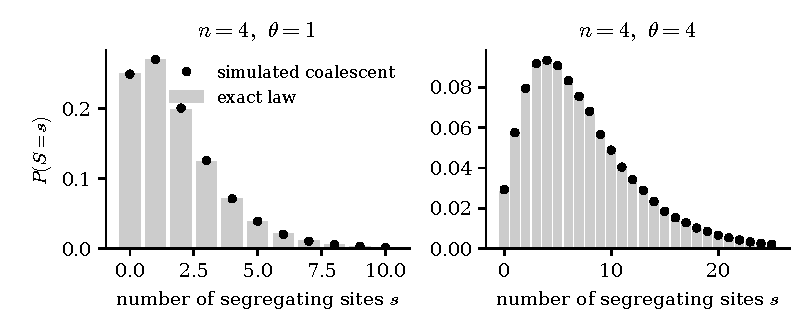
\includegraphics{figures/coal_pmf4.pdf}
\caption{Exact mass function of $S$ for $n=4$ (bars) against $10^5$ simulated coalescents with branch by branch mutation (points), at $\theta=1$ and $\theta=4$. The largest discrepancy is 0.0016.}
\label{coal:fig:pmf4}
\end{figure}

\begin{example}[No segregating sites]\label{coal:ex:zero}
The probability of a monomorphic sample is $\Prob(S=0)=\prod_{k=2}^np_k=(n-1)!/\{(\theta+1)(\theta+2)\cdots(\theta+n-1)\}$. At $\theta=1$ this is $1/n$, so among thirty sequences drawn from a population with $\theta=1$ there is a one in thirty chance of seeing no variation at all. The same expression is the Ewens probability that all $n$ genes carry one allele, which is the first sign of the coupling in Section~\ref{coal:sec:ewens}.
\end{example}

\subsection{Watterson's Estimator on a Small Sample}\label{coal:sec:wattex}

Theorem~\ref{coal:thm:geom} gives more than the moments of Watterson's estimator $\hat\theta_W=S/a_1(n)$: it gives an unbiased estimate of its variance and an exact confidence interval. Since $\E[S(S-1)]=\Var(S)+\E[S]^2-\E[S]=\theta^2\{a_1(n)^2+a_2(n)\}$, the statistic $S(S-1)/(a_1^2+a_2)$ is unbiased for $\theta^2$, and
\begin{equation}\label{coal:eq:varhat}
\widehat{\Var}(\hat\theta_W)=\frac{S}{a_1^2}+\frac{a_2}{a_1^2}\cdot\frac{S(S-1)}{a_1^2+a_2}
\end{equation}
is unbiased for $\Var(\hat\theta_W)=\theta/a_1+\theta^2a_2/a_1^2$. Because each $S_k$ is stochastically increasing in $\theta$, so is $S$, and an exact equal tailed $1-2\alpha$ interval is $[\theta_L,\theta_U]$ with $\Prob_{\theta_L}(S\ge s)=\alpha$ and $\Prob_{\theta_U}(S\le s)=\alpha$, both computed from \eqref{coal:eq:tavare}.

\begin{example}[A simulated sample of eleven sequences]\label{coal:ex:watterson}
Kreitman's classic survey of the alcohol dehydrogenase region in \emph{Drosophila melanogaster} sequenced eleven alleles \citep{coal:kreitman1983}, and we mimic its size with a clearly labelled simulation: $n=11$ sequences from the coalescent with $\theta=4$ (random seed 1983). The data matrix, with rows sorted and the derived allele written as 1, is
\begin{center}
\small\ttfamily
\begin{tabular}{l}
1111\,1\,0000\,0\,1\,0\,0000\,00\\
1111\,1\,0000\,0\,1\,0\,0000\,00\\
1111\,1\,0000\,0\,0\,0\,0000\,00\\
1111\,1\,0000\,0\,0\,0\,0000\,00\\
1111\,1\,0000\,0\,0\,0\,0000\,00\\
1111\,0\,0000\,0\,0\,1\,0000\,00\\
1111\,0\,0000\,0\,0\,0\,0000\,11\\
0000\,0\,1111\,1\,0\,0\,0000\,00\\
0000\,0\,1111\,1\,0\,0\,0000\,00\\
0000\,0\,1111\,1\,0\,0\,0000\,00\\
0000\,0\,1111\,0\,0\,0\,1111\,00
\end{tabular}
\end{center}
with columns grouped by their derived allele count. There are $S=18$ segregating sites with spectrum $\bm\xi=(7,1,1,4,1,0,4,0,0,0)$, and $H=6$ distinct haplotypes. With $a_1(11)=2.92897$ and $a_2(11)=1.54977$,
\[
\hat\theta_W=\frac{18}{2.92897}=6.15,\qquad \widehat{\Var}(\hat\theta_W)=7.56,\qquad \widehat{\mathrm{se}}=2.75.
\]
The normal interval $\hat\theta_W\pm1.645\,\widehat{\mathrm{se}}$ is $(1.62,10.67)$. The exact 90\% interval from the geometric law is $(2.97,15.05)$: it is shifted upward and is markedly asymmetric, because the law of $S$ is right skewed and its variance grows like $\theta^2$. The maximum likelihood estimate from $S$ alone is $6.49$, slightly above $\hat\theta_W$. Under the scale invariant prior $\pi(\theta)\propto1/\theta$ the exact posterior given $S$ has median 6.50 and 90\% interval $(2.97,14.31)$; under an exponential prior with mean 10 the median is 6.89 and the interval $(3.30,14.11)$. For comparison the mean pairwise difference is $\hat\theta_\pi=\binom{11}{2}^{-1}\sum_ii(11-i)\xi_i=6.65$ and Tajima's $D$ \citep{coal:tajima1989} is 0.37, unremarkable under neutrality. A repeated sampling check with $2\times10^4$ samples at $\theta=4$ gives mean $\hat\theta_W$ of 4.007, variance 4.267 against the theoretical 4.256, and mean of \eqref{coal:eq:varhat} 4.268, confirming unbiasedness.
\end{example}

The example also shows how little eleven sequences say about $\theta$. The exact interval spans a factor of five, and most of that width is the tree term $\theta^2a_2$, which no amount of additional sequence length removes. Only more sequences, or information about the tree beyond $S$, can narrow it, and the rest of the chapter is about the second route.

\subsection{A Coupling with the Ewens Sampling Formula}\label{coal:sec:ewens}

This section places Kingman's two models of neutral variation on one probability space. Kingman's other model for the same biology is the Ewens sampling formula, whose block count admits the Feller coupling $K_n=\sum_{i=1}^n B_i$ with $B_i\sim\coalBern\{\theta/(\theta+i-1)\}$ independent \citep{coal:ewens1972,coal:kingman1977}. Comparing this with \eqref{coal:eq:geom}, note that the geometric failure probability is
\begin{equation}\label{coal:eq:fail}
1-p_k=\frac{\theta}{\theta+k-1},
\end{equation}
which is exactly the Bernoulli success probability in the Feller coupling. The two models are built from the same sequence.

\begin{corollary}[Bernoulli geometric duality]\label{coal:cor:duality}
On a common probability space carrying $S_2,\dots,S_n$ as in Theorem~\ref{coal:thm:geom},
\begin{equation}\label{coal:eq:duality}
K_n \;\overset{d}{=}\; 1+\#\{\,k\in\{2,\dots,n\}: S_k\ge 1\,\},
\end{equation}
where $K_n$ is the number of blocks under the Ewens sampling formula with the same $\theta$.
\end{corollary}

\begin{proof}
$\Prob(S_k\ge1)=1-p_k=\theta/(\theta+k-1)$ by \eqref{coal:eq:fail}, and the $S_k$ are independent, so $\#\{k\ge2: S_k\ge1\}$ is a sum of independent $\coalBern\{\theta/(\theta+k-1)\}$ variables over $k=2,\dots,n$. The Feller coupling gives $K_n$ as the same sum over $i=1,\dots,n$, and the $i=1$ term is $\coalBern(1)\equiv1$.
\end{proof}

The interpretation is clean. Both models decompose the sample along the $n-1$ coalescent levels, and both attach an independent count to each level with the same parameter. Kingman's partition records only whether a level is marked; the coalescent records how many marks it carries. In law, the partition is the thresholded coalescent. Example~\ref{coal:ex:zero} is the case of no marks: $\Prob(S=0)=\Prob(K_n=1)$.

There is a second, more literal, link between the two models, and it involves the haplotype count.

\begin{proposition}[Haplotypes follow the Ewens formula]\label{coal:prop:hapewens}
Under the infinite sites model on Kingman's coalescent, the partition of the $n$ sequences into identical haplotypes has the law of the Ewens sampling formula with parameter $\theta$. In particular $H\overset{d}{=}K_n$, and $\E[H]=\sum_{i=1}^n\theta/(\theta+i-1)$.
\end{proposition}

\begin{proof}
Two sampled sequences are identical exactly when no mutation falls on the path joining them in the genealogy, since every mutation on that path creates a site at which one carries the derived allele and the other does not, and mutations off the path affect both or neither. Now place the infinite alleles model on the same genealogy and the same mutation events, so that each mutation creates a new allele inherited by its descendants. Two genes then carry the same allele exactly when neither has a mutation on its line of descent below their most recent common ancestor, which is again the condition that the joining path is free of mutations. The two partitions therefore coincide pathwise. The allelic partition of the infinite alleles model on the coalescent has the Ewens law \citep{coal:ewens1972,coal:kingman1982}, and the block count of the Ewens formula has mean $\sum_i\theta/(\theta+i-1)$ by the Feller coupling.
\end{proof}

So $H$ and the thresholded count $K'=1+\#\{k:S_k\ge1\}$ have the same law, but they are different random variables: $H$ is a function of the data, while $K'$ is not, since the data do not reveal in which epoch a mutation arose.

\begin{example}[The coupling for four sequences]\label{coal:ex:coupling}
Take $n=4$ and $\theta=1$. The Ewens law of $K_4$ is $|s(4,k)|/4!$, where $s$ denotes Stirling numbers of the first kind, giving $6/24$, $11/24$, $6/24$ and $1/24$ for $k=1,2,3,4$. The thresholded coalescent marks levels $2,3,4$ independently with probabilities $1/2$, $1/3$, $1/4$, so $\Prob(K'=1)=\tfrac12\cdot\tfrac23\cdot\tfrac34=\tfrac14$ and $\Prob(K'=4)=\tfrac12\cdot\tfrac13\cdot\tfrac14=\tfrac1{24}$, in agreement. In the $2\times10^5$ coalescents of Example~\ref{coal:ex:n4} the frequencies of $K'$ are 0.2514, 0.4562, 0.2515, 0.0409 and those of $H$ are 0.2514, 0.4562, 0.2509, 0.0414, against the exact 0.2500, 0.4583, 0.2500, 0.0417. Yet $K'\ne H$ in 13.7\% of samples. Table~\ref{coal:tab:joint} shows the joint law: the two agree whenever there is no mutation at all, and otherwise may disagree in either direction. For instance a mutation on lineage $c$ in the three lineage epoch followed by a second mutation on the same lineage in the two lineage epoch gives $K'=3$ but only $H=2$, since both derived alleles are carried by one sequence.

The coupling also says how many sites to expect given the partition. Given $K'$, the marked levels carry $1+\coalGeom(p_k)$ sites by the memoryless property, with mean $1/p_k$. With only one level marked, the mark sits on level $2$, $3$ or $4$ with probabilities proportional to $\tfrac14$, $\tfrac18$, $\tfrac1{12}$, so
\[
\E[S\mid K'=2]=\frac{\tfrac14\cdot2+\tfrac18\cdot\tfrac32+\tfrac1{12}\cdot\tfrac43}{\tfrac{11}{24}}=\frac{115}{66}=1.742,
\]
against 1.744 in simulation; similarly $\E[S\mid K'=3]=10/3$ and $\E[S\mid K'=4]=29/6$.
\end{example}

\begin{table}[t]
\centering
\small
\begin{tabular}{ccccc}
\toprule
 & $H=1$ & $H=2$ & $H=3$ & $H=4$\\
\midrule
$K'=1$ & 0.2514 & 0 & 0 & 0\\
$K'=2$ & 0 & 0.4081 & 0.0458 & 0.0024\\
$K'=3$ & 0 & 0.0467 & 0.1846 & 0.0202\\
$K'=4$ & 0 & 0.0014 & 0.0206 & 0.0189\\
\bottomrule
\end{tabular}
\caption{Joint frequencies of the thresholded level count $K'=1+\#\{k:S_k\ge1\}$ and the haplotype count $H$ in $2\times10^5$ coalescents with $n=4$, $\theta=1$. Both margins follow the Ewens law, but the variables differ in 13.7\% of samples.}
\label{coal:tab:joint}
\end{table}

In the eleven sequence sample of Example~\ref{coal:ex:watterson}, mutations fell in seven of the ten epochs, so $K'=8$, while the data show $H=6$ haplotypes.

The duality also settles how much is lost by thresholding. Both statistics are sufficient for $\theta$ within their own reduced models, so their Fisher informations are computable.

\begin{proposition}[Information]\label{coal:prop:info}
Let $I_K(\theta)$ be the Fisher information about $\theta$ in the Ewens block count and $I_{\bm S}(\theta)$ that in the full levelwise vector $(S_2,\dots,S_n)$. Then
\begin{equation}\label{coal:eq:info}
I_K(\theta)=\frac1\theta\sum_{k=2}^n\frac{k-1}{(\theta+k-1)^2},\qquad
I_{\bm S}(\theta)=\frac1\theta\sum_{k=2}^n\frac{1}{\theta+k-1},
\end{equation}
so $I_K(\theta)\le I_{\bm S}(\theta)$ with per term ratio $(k-1)/(\theta+k-1)\uparrow1$, and both satisfy $I(\theta)=\theta^{-1}\log n+O(1)$ as $n\to\infty$ for fixed $\theta$.
\end{proposition}

\begin{proof}
By the Ewens sampling formula the law of $K_n$ is $\Prob_\theta(K_n=k)=|s(n,k)|\theta^k/\{\theta(\theta+1)\cdots(\theta+n-1)\}$, a one parameter exponential family with natural parameter $\eta=\log\theta$ and sufficient statistic $k$. The information in $\eta$ is therefore $\Var_\theta(K_n)$, and the information in $\theta$ is $\Var_\theta(K_n)(d\eta/d\theta)^2=\theta^{-2}\sum_i q_i(1-q_i)$ with $q_i=\theta/(\theta+i-1)$, using the Feller coupling for the variance. Since $q_i(1-q_i)=\theta(i-1)/(\theta+i-1)^2$, and the $i=1$ term vanishes, the first identity follows.

For the second, write a geometric on $\{0,1,\dots\}$ with mean $m$ as $\Prob(j)=(1+m)^{-1}\{m/(1+m)\}^j$. The score in $m$ is $j/m-(j+1)/(1+m)=(j-m)/\{m(1+m)\}$, and since $\Var(j)=m(1+m)$ the information in $m$ is $\{m(1+m)\}^{-1}$. Here $m_k=\theta/(k-1)$, so $dm_k/d\theta=1/(k-1)$, and the information about $\theta$ in $S_k$ is $(k-1)^{-2}\{m_k(1+m_k)\}^{-1}=\{\theta(\theta+k-1)\}^{-1}$. Independence makes information additive, which gives the second identity.

The per term ratio of the two sums is $(k-1)/(\theta+k-1)<1$. For the asymptotics, $\sum_{k=2}^n(\theta+k-1)^{-1}=\log n+O(1)$ by comparison with $a_1(n)$, since the difference of the two sums is bounded by $\theta\, a_2(n)\le\theta\pi^2/6$. Likewise $\sum_{k=2}^n(k-1)/(\theta+k-1)^2=\sum_k(\theta+k-1)^{-1}-\theta\sum_k(\theta+k-1)^{-2}=\log n+O(1)$.
\end{proof}

Proposition~\ref{coal:prop:info} says the partition and the genealogy learn $\theta$ at the same leading rate, $\theta^{-1}\log n$, even though the coalescent count has strictly larger variance. Larger variance is not less information here, because the mean grows differently; the ordering that does hold, $I_K\le I_{\bm S}$, is a data processing consequence of the thresholding in \eqref{coal:eq:duality}. The levelwise vector is not observed, however, and the observed count $S$ is a coarsening of it, so the question is where $S$ itself sits.

\begin{corollary}[Information in $S$]\label{coal:cor:infoS}
The Fisher information $I_S(\theta)$ in the observed count $S$ satisfies
\[
\frac{a_1(n)^2}{\theta a_1(n)+\theta^2a_2(n)}\;\le\;I_S(\theta)\;\le\;I_{\bm S}(\theta),
\]
and therefore $I_S(\theta)=\theta^{-1}\log n+O(1)$. By Proposition~\ref{coal:prop:hapewens} the haplotype count carries exactly $I_K(\theta)$.
\end{corollary}

\begin{proof}
The upper bound holds because $S$ is a function of $(S_2,\dots,S_n)$ and Fisher information cannot increase under a measurable map. The lower bound is the Cram\'er and Rao inequality applied to the unbiased estimator $\hat\theta_W=S/a_1$, whose variance is $\theta/a_1+\theta^2a_2/a_1^2$ by \eqref{coal:eq:watterson}; the family of laws of $S$ is smooth in $\theta$, being a finite signed combination of geometric terms by \eqref{coal:eq:tavare}. The lower bound equals $\theta^{-1}a_1-a_2/(1+\theta a_2/a_1)\ge\theta^{-1}a_1-a_2$, and the upper bound is at most $\theta^{-1}a_1$, so both are $\theta^{-1}\log n+O(1)$.
\end{proof}

\begin{table}[t]
\centering
\small
\begin{tabular}{rrccccc}
\toprule
$n$ & $\theta$ & $I_K=I_H$ & $1/\Var(\hat\theta_W)$ & $I_S$ & $I_{\bm S}$ & $\theta^{-1}\log n$\\
\midrule
4 & 1 & 0.660 & 1.052 & 1.053 & 1.083 & 1.386\\
4 & 5 & 0.023 & 0.078 & 0.078 & 0.087 & 0.277\\
30 & 1 & 2.383 & 2.816 & 2.824 & 2.995 & 3.401\\
30 & 5 & 0.215 & 0.261 & 0.270 & 0.367 & 0.680\\
500 & 1 & 5.150 & 5.468 & 5.479 & 5.793 & 6.215\\
500 & 5 & 0.724 & 0.615 & 0.638 & 0.903 & 1.243\\
\bottomrule
\end{tabular}
\caption{Fisher information about $\theta$ in the Ewens block count (equivalently the haplotype count), in Watterson's estimator, in the exact law of $S$, and in the unobserved levelwise vector. $I_S$ is computed from the exact mass function by numerical differentiation.}
\label{coal:tab:info}
\end{table}

Table~\ref{coal:tab:info} puts numbers on these bounds. Watterson's estimator is nearly efficient for the law of $S$, losing at most 4\% of $I_S$ in these cases, so little is gained by replacing it with the maximum likelihood estimate from $S$. The logarithmic asymptotics are slow: even at $n=500$ the leading term exceeds each of $I_K$, $I_S$ and $I_{\bm S}$ by between 7\% and 95\%. And the ordering between the two observable scalars is not fixed. At small $\theta$ the count $S$ is more informative than $H$, but at $n=500$ and $\theta=5$ the haplotype count carries 0.724 against 0.638 for $S$, because the tree variance $\theta^2a_2$ that inflates $\Var(S)$ affects a thresholded count much less. This is an early hint that $S$ and $H$ see different aspects of the genealogy.

\section{Sufficiency Fails}\label{coal:sec:suff}

This section shows that the coalescent has no analogue of the block count. For the Ewens model the block count is exactly sufficient, which is what made generative computation trivial in Chapter~\ref{ch:suff}. The obstruction is structural rather than technical: the data are informative about a latent tree whose law, after conditioning on $S$, still depends on $\theta$.

\begin{proposition}[$S$ is not sufficient for $\theta$]\label{coal:prop:notsuff}
Let $X$ denote the full infinite sites data and $G$ the genealogy. Then
\begin{equation}\label{coal:eq:lik}
p(X\mid\theta)\;=\;\Bigl(\frac\theta2\Bigr)^{S(X)}\int e^{-\theta L_G/2}\,w(X,G)\,\mu(dG),
\end{equation}
where $w$ and the genealogy law $\mu$ are free of $\theta$. The conditional law of $X$ given $S$ depends on $\theta$ unless the measures $w(X,G)\mu(dG)$, pushed forward to $L_G$, are proportional across configurations with equal $S$. For $n=3$ and $n=4$ they are not, so $S$ is not sufficient.
\end{proposition}

\begin{proof}
Conditionally on $G$, the mutations form a Poisson process of rate $\theta/2$ on a tree of total length $L_G$. The probability that branch $b$ of length $t_b$ receives exactly $m_b$ mutations for every $b$ is $\prod_be^{-\theta t_b/2}(\theta t_b/2)^{m_b}/m_b!=e^{-\theta L_G/2}(\theta/2)^{S}\prod_bt_b^{m_b}/m_b!$ with $S=\sum_bm_b$, and summing over the placements compatible with $X$ gives a factor $w(X,G)$ that does not involve $\theta$. Integrating over $\mu$ gives \eqref{coal:eq:lik}. Sufficiency of $S$ would require the ratio of \eqref{coal:eq:lik} for two configurations $X,X'$ with $S(X)=S(X')$ to be constant in $\theta$. That ratio is
\[
\frac{\int e^{-\theta L_G/2}w(X,G)\mu(dG)}{\int e^{-\theta L_G/2}w(X',G)\mu(dG)},
\]
the ratio of two Laplace transforms in $\theta/2$ of the image measures of $w(X,G)\mu(dG)$ and $w(X',G)\mu(dG)$ under $G\mapsto L_G$. By uniqueness of the Laplace transform it is constant in $\theta$ only if these two measures on $(0,\infty)$ are proportional, that is, only if $\E_\mu[w(X,G)\mid L_G]$ and $\E_\mu[w(X',G)\mid L_G]$ have a constant ratio. Example~\ref{coal:ex:n3} exhibits configurations at $n=3$ for which they do not, and Example~\ref{coal:ex:samesfs} does the same at $n=4$. For larger samples we do not give a general argument, but the same tilt is at work and Section~\ref{coal:sec:exp} detects its consequences at $n=30$.
\end{proof}

\begin{example}[A minimal failure of sufficiency]\label{coal:ex:n3}
Take $n=3$ and condition on a single segregating site, $S=1$. Label the first pair to merge $a,b$ and the remaining lineage $c$. The external branches of $a$ and $b$ have length $T_3$, that of $c$ has length $T_3+T_2$, and the internal branch above $\{a,b\}$ has length $T_2$, so $L_3=3T_3+2T_2$. The single site is a doubleton, with derived allele in two sequences, exactly when the mutation falls on the internal branch. By \eqref{coal:eq:lik} with $s=1$,
\[
\Prob_\theta(\xi_2=1\mid S=1)=\frac{\E\bigl[T_2e^{-\theta L_3/2}\bigr]}{\E\bigl[L_3e^{-\theta L_3/2}\bigr]}.
\]
With $T_3\sim\coalExp(3)$ and $T_2\sim\coalExp(1)$ independent, $\E[e^{-3\theta T_3/2}]=(1+\theta/2)^{-1}$, $\E[T_3e^{-3\theta T_3/2}]=\{3(1+\theta/2)^2\}^{-1}$, $\E[e^{-\theta T_2}]=(1+\theta)^{-1}$ and $\E[T_2e^{-\theta T_2}]=(1+\theta)^{-2}$. Hence the numerator is $(1+\theta/2)^{-1}(1+\theta)^{-2}$ and the denominator is $(1+\theta/2)^{-2}(1+\theta)^{-1}+2(1+\theta/2)^{-1}(1+\theta)^{-2}$. Multiplying both by $(1+\theta/2)^2(1+\theta)^2$,
\[
\Prob_\theta(\xi_2=1\mid S=1)=\frac{1+\theta/2}{(1+\theta)+2(1+\theta/2)}=\frac{2+\theta}{2(3+2\theta)}.
\]
This decreases from $1/3$ at $\theta\to0$, where it is the ratio $\E[\ell_2]/\E[L_3]=1/3$ of expected branch lengths, to $1/4$ as $\theta\to\infty$. At $\theta=0.5$, $2$ and $8$ it equals 0.3125, 0.2857 and 0.2632, and the fractions of doubletons among simulated samples with $S=1$ are 0.3147, 0.2871 and 0.2632, each within 1.2 standard errors. So whether the one segregating site is shared by two sequences or carried by one is informative about $\theta$ beyond the fact that there is one site: a doubleton points to a long internal branch, hence a long tree, hence a smaller $\theta$ for the same number of mutations.
\end{example}

The point is worth stating in words. Conditioning on the number of mutations leaves behind a tilt $e^{-\theta L_G/2}$ on the tree, and the configuration $X$ is informative about the tree. So learning where the mutations fell tells us something about $\theta$ beyond how many there were. Watterson's estimator, which uses $S$ alone, is unbiased but discards this, which is the source of its inefficiency relative to the full likelihood noted by \citet{coal:felsenstein1992}.

\begin{remark}[Contrast]\label{coal:rem:contrast}
In the Ewens model the analogous tilt is absent because the partition is generated directly, with no latent tree to integrate. This is the precise sense in which Kingman's two models differ for inference, despite Corollary~\ref{coal:cor:duality} placing them on one probability space.
\end{remark}

Section~\ref{coal:sec:exp} quantifies the loss at realistic sizes: at $n=30$ with constant population size, moving from $S$ to the spectrum narrows the 90\% posterior interval for $\theta$ from 84.1 to 64.1.

\section{A Ceiling on Learned Summaries}\label{coal:sec:ceiling}

If the summary cannot be derived it must be learned, and the standard device is a permutation invariant encoder of DeepSets type \citep{coal:zaheer2017}, applied to the multiset of sites. This section establishes in advance what such an encoder can and cannot see.

\begin{definition}\label{coal:def:deepsets}
An encoder $e$ is of \emph{per site DeepSets form} if $e(X)=\rho\bigl(\sum_{j=1}^S\phi(x_j)\bigr)$ for the columns $x_1,\dots,x_S$ of $X$, with $\phi$ invariant under permutation of the $n$ lineages.
\end{definition}

Per site invariance of $\phi$ is the natural way to impose exchangeability of lineages, since the labelling of sampled individuals is arbitrary and the same relabelling applies to every site. The sum over sites makes $e$ invariant under permutation of sites as well. The theorem below says these two natural symmetries, imposed site by site, throw away everything except allele frequencies.

\begin{theorem}[DeepSets encoders factor through the spectrum]\label{coal:thm:deepsets}
Every encoder of per site DeepSets form satisfies
\begin{equation}\label{coal:eq:factor}
e(X)\;=\;\rho\Bigl(\sum_{i=1}^{n-1}\xi_i\,\tilde\phi(i)\Bigr)
\end{equation}
for some $\tilde\phi$, and is therefore a function of the site frequency spectrum $\bm{\xi}$ alone.
\end{theorem}

\begin{proof}
A function of $x\in\{0,1\}^n$ invariant under all permutations of the $n$ coordinates depends on $x$ only through $|x|=\sum_l x_l$, since any two binary vectors of the same weight are related by a permutation. Hence $\phi(x_j)=\tilde\phi(|x_j|)$ where $|x_j|$ is the derived allele count at site $j$, which lies in $\{1,\dots,n-1\}$ because site $j$ is segregating. Grouping the sum over sites by that count gives $\sum_j\tilde\phi(|x_j|)=\sum_{i=1}^{n-1}\xi_i\tilde\phi(i)$, and \eqref{coal:eq:factor} follows.
\end{proof}

The theorem is a statement about architecture, so it holds whatever $\rho$ is and however the network is trained. Its genetic content is that a per site encoder sees each site's allele frequency and nothing about which sequences share which alleles.

\begin{corollary}[The spectrum is a strict coarsening]\label{coal:cor:coarse}
Under the infinite sites model without recombination, the maximal invariant of $X$ under relabelling of lineages and permutation of sites is the gene tree, that is, the unlabelled rooted topology with mutation counts on its edges. The spectrum $\bm{\xi}$ is a strict coarsening of it. Consequently no per site DeepSets encoder, at any depth or width, can recover the information in $X$ that is not already in $\bm{\xi}$.
\end{corollary}

\begin{proof}
Under infinite sites without recombination, the sets of sequences carrying the derived allele at the various sites are pairwise nested or disjoint, and the perfect phylogeny they determine is the gene tree. Relabelling lineages and permuting sites preserve these nesting relations and the number of sites with each carrier set, so the gene tree is invariant. Conversely, the gene tree determines $X$ up to an assignment of sequence labels to its leaves and an ordering of its sites, so two matrices with the same gene tree differ by a relabelling and a permutation of sites. That $\bm{\xi}$ is strictly coarser is seen already at $n=4$ with two segregating sites, each carrying a single derived allele, so that $\xi_1=2$. If both mutations fall on the same external branch the gene tree has one doubly mutated tip; if they fall on different external branches it has two singly mutated tips. The spectra are identical and the gene trees are not. The final claim is Theorem~\ref{coal:thm:deepsets}.
\end{proof}

Corollary~\ref{coal:cor:coarse} is a limitation of an architecture class, not of the data, and it is useful precisely because per site DeepSets encoders are the default choice. To show that the ceiling matters one needs a statistic that is computable, invariant, and provably outside the reach of \eqref{coal:eq:factor}. The classical choice is the number of distinct haplotypes.

\begin{proposition}[Haplotype count escapes the spectrum]\label{coal:prop:hap}
The haplotype count $H=H(X)$ is invariant under relabelling of lineages and under permutation of sites, and $H$ is not a function of $\bm{\xi}$.
\end{proposition}

\begin{proof}
Invariance is immediate, since permuting rows permutes the multiset of rows and permuting columns applies a fixed bijection to every row. For the second claim take the configuration of Corollary~\ref{coal:cor:coarse}, with $n=4$ and $\xi_1=2$. If both mutations lie on the same external branch, the rows are $(1,1)$ for that tip and $(0,0)$ for the other three, so $H=2$. If they lie on different external branches, the rows are $(1,0)$, $(0,1)$ and $(0,0)$ twice, so $H=3$. The spectra coincide.
\end{proof}

Proposition~\ref{coal:prop:hap} identifies $H$ as a minimal witness that the spectrum is lossy: it is not a per site feature, since it depends on which lineages share which mutations, so no encoder of the form \eqref{coal:eq:factor} computes it. The next example shows that the information it carries changes the posterior, not merely the data.

\begin{example}[Same spectrum, different posteriors]\label{coal:ex:samesfs}
Take $n=4$ and the two data sets of Proposition~\ref{coal:prop:hap}: in data set A one sequence carries both derived alleles ($H=2$); in data set B two sequences carry one each ($H=3$). Both have $\bm\xi=(2,0,0)$. Let $e_1,\dots,e_4$ be the external branch lengths. By the Poisson placement in the proof of Proposition~\ref{coal:prop:notsuff}, up to factors free of $\theta$,
\[
p(\mathrm A\mid\theta)\propto\theta^2\,\E\Bigl[e^{-\theta L_4/2}\sum_j\tfrac12e_j^2\Bigr],\qquad
p(\mathrm B\mid\theta)\propto\theta^2\,\E\Bigl[e^{-\theta L_4/2}\sum_{i<j}e_ie_j\Bigr],
\]
with the same constant of proportionality, so that $p(\mathrm A\mid\theta)+p(\mathrm B\mid\theta)$ is the probability of the spectrum. Two topologies occur. With probability $2/3$ the tree is a caterpillar with $(e_1,\dots,e_4)=(T_4,T_4,T_4+T_3,T_4+T_3+T_2)$, and with probability $1/3$ it is balanced with $(T_4,T_4,T_4+T_3,T_4+T_3)$; in both $L_4=4T_4+3T_3+2T_2$. The expectations reduce to the tilted exponential moments $\E[T_k^me^{-\theta kT_k/2}]=m!\,\lambda_k/\mu_k^{m+1}$ with $\mu_k=k(k-1+\theta)/2$, so the likelihoods are explicit rational functions of $\theta$.

The conditional probability of A given the spectrum is 0.489, 0.457, 0.434, 0.409, 0.388 and 0.373 at $\theta=0.1$, $0.5$, $1$, $2$, $4$, $8$, tending to $1/2$ as $\theta\to0$. Simulation agrees: among coalescents with $\bm\xi=(2,0,0)$ the fraction with $H=2$ is 0.433 at $\theta=1$ (21708 samples) and 0.389 at $\theta=4$ (9961 samples). The maximum likelihood estimates are 1.13 from A, 1.30 from B and 1.22 from the spectrum alone, and under a $\coalGa(2,1)$ prior the posterior means are 1.71, 1.80 and 1.76. The data sets agree in every per site summary and disagree about $\theta$. The direction makes sense: a larger $\theta$ tilts toward shorter trees, the tilt shrinks the deep epochs most, the external branches become more nearly equal, and two mutations are then more likely to land on different tips.
\end{example}

Capturing linkage more fully requires either features defined on pairs of sites, so that $\phi$ is no longer per site invariant while $e$ remains invariant overall, or an architecture defined on the inferred gene tree. A pairwise feature already separates the two data sets of Example~\ref{coal:ex:samesfs}: the number of pairs of identical columns is one in A and zero in B. We take only the scalar step here. What Corollary~\ref{coal:cor:coarse} buys is an interpretation of our own results: spectrum based posteriors are the ceiling for the DeepSets class, and Section~\ref{coal:sec:hap} measures how much a statistic above the ceiling adds in practice.

\section{Generative Bayesian Computation}\label{coal:sec:gbc}

This section recalls the transport map formulation of Chapter~\ref{ch:suff} in the form used for the experiments, and records the simulator.

\subsection{The Quantile Map}\label{coal:sec:quantile}

Let $\vartheta\sim\pi$ be the parameter, $X\sim p(\cdot\mid\vartheta)$ the data, and $Z=e(X)$ an encoding. Generative Bayesian computation (GBC) seeks a map $\mathcal{Q}$ with
\begin{equation}\label{coal:eq:transport}
\vartheta\;\overset{d}{=}\;\mathcal{Q}(Z,U)\mid Z,\qquad U\sim\coalUnif(0,1)\;\perp\!\!\!\perp\;Z,
\end{equation}
so that posterior draws are evaluations at fresh uniforms. For scalar $\vartheta$, $\mathcal{Q}(Z,\cdot)$ is the posterior quantile function, characterised as the minimiser of expected check loss,
\begin{equation}\label{coal:eq:check}
\begin{gathered}
\mathcal{Q}=\arg\min_h\;\E_{\pi(\vartheta)p(X\mid\vartheta)}\E_U\bigl[\rho_U\{\vartheta-h(Z,U)\}\bigr],\\
\rho_u(r)=r\{u-\coalind(r<0)\}.
\end{gathered}
\end{equation}
The expectation is over the prior predictive, which we can sample from without evaluating any likelihood. That is the entire appeal for the coalescent. Since quantiles commute with increasing maps, we fit the quantile function of $\log\vartheta$ and exponentiate.

\subsection{Vector Parameters}\label{coal:sec:vector}

For $\vartheta=(\vartheta_1,\vartheta_2)$ the check loss applied coordinatewise recovers the two \emph{marginal} posterior quantile functions, not the joint law. The joint is obtained autoregressively,
\begin{equation}\label{coal:eq:autoreg}
\vartheta_1=\mathcal{Q}_1(Z,U_1),\qquad\vartheta_2=\mathcal{Q}_2(Z,\vartheta_1,U_2),
\end{equation}
with $\mathcal{Q}_2$ trained by the same objective on the augmented input. In Section~\ref{coal:sec:exp} we report marginals, which is what \eqref{coal:eq:check} delivers directly, and we do not evaluate the joint map \eqref{coal:eq:autoreg}.

\subsection{Algorithm}\label{coal:sec:algorithm}

\begin{center}
\begin{minipage}{\textwidth}
\hrule\smallskip
Algorithm \thechapter.1\quad GBC for coalescent parameters
\smallskip\hrule
\begin{enumerate}[label={\footnotesize\arabic*:},leftmargin=2em,itemsep=1pt,topsep=3pt]
\item Input: sample size $n$, prior $\pi$, encoder $e$, training size $N$, network $h_\phi$.
\item for $r=1,\dots,N$ do
\item \quad draw $\vartheta^{(r)}\sim\pi$;
\item \quad draw coalescent times $T_k\sim\coalExp\{k(k-1)/2\}$ and merge uniformly chosen pairs, accumulating $\ell_i$, the branch length subtending $i$ leaves;
\item \quad draw $\xi_i^{(r)}\sim\coalPois(\theta^{(r)} \ell_i/2)$ for $i=1,\dots,n-1$ and set $Z^{(r)}=e(\bm{\xi}^{(r)})$.
\item end for
\item Minimise the empirical check loss over minibatches, drawing $u\sim\coalUnif(\epsilon,1-\epsilon)$ afresh at each step.
\item Output: for observed $Z$, posterior draws $\{h_{\hat\phi}(Z,u^{(m)})\}$, sorted in $u$.
\end{enumerate}
\hrule
\end{minipage}
\end{center}

\begin{sloppypar}Under exponential growth with $N(t)=N_0e^{-gt}$ backwards in time, step 4 is modified by the standard time change. The coalescence intensity at time $t$ is proportional to $1/N(t)\propto e^{gt}$, so the coalescent runs at constant rate in the rescaled time $\Lambda(t)=\int_0^te^{gs}ds=(e^{gt}-1)/g$. We therefore generate the coalescent in rescaled time and map back by $t=g^{-1}\log(1+g\Lambda)$. The encoder input is $\log(1+\xi_i)$, standardised.\end{sloppypar}

\section{Experiments}\label{coal:sec:exp}

The experiments grade learned posteriors against exact ones wherever the theory of Sections~\ref{coal:sec:model} to~\ref{coal:sec:ceiling} supplies an exact answer, and measure what the spectrum and the haplotype count add where it does not. Throughout $n=30$, so the spectrum has 29 cells. Networks have two hidden layers of 128 rectified linear units, trained by Adam on the check loss with a decaying learning rate. As a check on the simulator, at $g=0$ and $\theta=8$ the simulated spectrum means over $2\times10^4$ replicates are 8.047, 4.014, 2.628, 1.567, 0.796 at $i=1,2,3,5,10$, against the theoretical $\theta/i$ values 8, 4, 2.667, 1.6, 0.8.

\begin{table}[t]
\centering
\small
\setlength{\tabcolsep}{4.5pt}
\begin{tabular}{clrrrrr}
\toprule
$S$ & method & 5\% & 25\% & 50\% & 75\% & 95\%\\
\midrule
20 & exact & 3.392 & 4.760 & 5.962 & 7.407 & 9.992\\
   & GBC   & 3.410 & 4.759 & 5.936 & 7.370 & 9.771\\
40 & exact & 6.063 & 8.210 & 10.038 & 12.180 & 15.892\\
   & GBC   & 6.122 & 8.206 & 9.987 & 12.106 & 15.620\\
60 & exact & 8.268 & 11.028 & 13.355 & 16.048 & 20.641\\
   & GBC   & 8.330 & 10.947 & 13.368 & 16.055 & 20.479\\
90 & exact & 10.977 & 14.437 & 17.343 & 20.685 & 26.316\\
   & GBC   & 11.144 & 14.312 & 17.285 & 20.471 & 26.288\\
\bottomrule
\end{tabular}
\caption{Posterior quantiles of $\theta$ given the number of segregating sites at $n=30$ under a $\coalGa(3,3)$ prior. Exact values by inversion of the generating function of Theorem~\ref{coal:thm:geom} followed by quadrature; GBC values from the trained quantile network.}
\label{coal:tab:exact}
\end{table}

\begin{table}[t]
\centering
\small
\setlength{\tabcolsep}{3pt}
\begin{tabular}{lccc}
\toprule
encoder & \begin{tabular}[b]{@{}c@{}}mean 90\%\\ width for $\theta$\end{tabular} & \begin{tabular}[b]{@{}c@{}}coverage\\ at 90\%\end{tabular} & \begin{tabular}[b]{@{}c@{}}coverage\\ at 50\%\end{tabular}\\
\midrule
site frequency spectrum & 64.09 & 0.886 & 0.450\\
$S$ alone & 84.15 & 0.896 & 0.497\\
prior & 159.68 & {} & {}\\
\bottomrule
\end{tabular}
\caption{Constant population size, $n=30$, $\pi(\theta)=\coalGa(4,\text{scale }25)$, $\E[S]=396$. The spectrum removes 60\% of the prior interval width against 47\% for $S$ alone, confirming Proposition~\ref{coal:prop:notsuff} numerically.}
\label{coal:tab:const}
\end{table}

\subsection{Exact Validation: the Posterior Given \texorpdfstring{$S$}{S}}\label{coal:sec:valS}

Corollary~\ref{coal:cor:exact} makes the posterior for $\theta$ given $S$ exactly computable, so we can grade the learned map rather than merely inspect it. We take $\pi(\theta)=\coalGa(3,\text{scale }3)$, train on $N=2\times10^5$ prior predictive pairs, and compare against quadrature on \eqref{coal:eq:post}.

Table~\ref{coal:tab:exact} shows that the largest discrepancy among the five tabulated quantiles is 0.22, 0.27, 0.16 and 0.21 at $S=20,40,60,90$. Over a grid of 49 levels spanning $[0.02,0.98]$ the maximum absolute discrepancies are 0.216, 0.305, 0.257 and 0.752, mean 0.383. Posterior standard deviations across these cases run from about 2 to 4.7, so the error is between 7 and 16 percent of a posterior standard deviation. Training noise matters at this scale: over four training seeds the grid maximum ranges from 0.06 to 1.40, that is from 3 to 30 percent of a posterior standard deviation, and its largest values sit at the extreme levels 0.02 and 0.98. For every seed it is largest at $S=90$, where the prior predictive thins in the upper tail.

\subsection{The Spectrum Beats \texorpdfstring{$S$}{S} at Constant Population Size}\label{coal:sec:beats}

Proposition~\ref{coal:prop:notsuff} says $S$ discards information about $\theta$ even when the population size is constant. We test this directly by training two networks on the same $9\times10^4$ replicates at $g\equiv0$ with $\pi(\theta)=\coalGa(4,\text{scale }25)$, one encoding the full spectrum and one encoding $S$ alone, and evaluating on $1.2\times10^4$ fresh replicates.

\begin{table}[t]
\centering
\small
\setlength{\tabcolsep}{3.5pt}
\begin{tabular}{llccc}
\toprule
encoder & parameter & \begin{tabular}[b]{@{}c@{}}mean 90\%\\ width\end{tabular} & \begin{tabular}[b]{@{}c@{}}coverage\\ at 90\%\end{tabular} & \begin{tabular}[b]{@{}c@{}}coverage\\ at 50\%\end{tabular}\\
\midrule
spectrum & $\theta$ & 74.83 & 0.885 & 0.447\\
spectrum & $g$ & 12.16 & 0.879 & 0.466\\
$S$ alone & $\theta$ & 95.59 & 0.903 & 0.507\\
$S$ alone & $g$ & 15.51 & 0.901 & 0.502\\
prior & $\theta$ & 159.68 & {} & {}\\
prior & $g$ & 18.00 & {} & {}\\
\bottomrule
\end{tabular}
\caption{Exponential growth, $n=30$, $\E[S]=142$. The spectrum removes 32\% of the prior width for the growth rate against 14\% for $S$ alone.}
\label{coal:tab:growth}
\end{table}

Table~\ref{coal:tab:const} is a direct numerical demonstration of Proposition~\ref{coal:prop:notsuff}. Were $S$ sufficient, the two rows would agree up to training error; instead the spectrum delivers an interval 24\% narrower. The gap is far larger than the discrepancies in Table~\ref{coal:tab:exact}, so it is not an artefact of optimisation. Part of it is miscalibration, since the spectrum row covers 0.886 against a nominal 0.90, but an interval that is 24\% narrower would need far worse coverage than this to be explained by overconfidence alone: shrinking a calibrated normal 90\% interval by 24\% cuts its coverage to about 0.79.

\subsection{Exponential Growth}\label{coal:sec:growth}

With a growth rate $g$ the model has two parameters and no closed form likelihood. We take $\pi(\theta)=\coalGa(4,\text{scale }25)$ and $g\sim\coalUnif(0,20)$, train on $1.2\times10^5$ replicates, and evaluate on $1.2\times10^4$ fresh ones. The mean number of segregating sites is 142.

The pattern in Table~\ref{coal:tab:growth} is what the theory predicts. The number of segregating sites is informative about the product of mutation rate and tree length, so it cannot separate a high mutation rate on a short tree from a low rate on a long one; it removes only 14\% of the prior width for $g$. The shape of the spectrum resolves the confounding, because growth skews the genealogy toward starlike topologies and hence toward an excess of singletons, and it removes 32\%. The improvement for $\theta$ is of similar size, consistent with Table~\ref{coal:tab:const}.

\subsection{Testing the Ceiling with Haplotype Structure}\label{coal:sec:hap}

Proposition~\ref{coal:prop:hap} supplies a statistic outside the DeepSets class, and this section measures what it adds. We track $H$ exactly during simulation by a merge recursion. For each node $v$ of the genealogy let $c_v$ be the number of distinct haplotypes among the leaves below $v$, and let $\alpha_v\in\{0,1\}$ record whether some leaf below $v$ carries exactly the sequence of $v$ itself, that is, has no mutation on its path up to $v$. Leaves have $c=\alpha=1$. When $A$ and $B$ merge into $C$, write $f_A$ for the indicator that the branch from $A$ up to $C$ carries no mutation, which has probability $e^{-\theta b_A/2}$ for a branch of length $b_A$, and similarly $f_B$. Then
\begin{equation}\label{coal:eq:merge}
c_C = c_A + c_B - \alpha_A\alpha_Bf_Af_B,\qquad \alpha_C=\max(\alpha_Af_A,\ \alpha_Bf_B),
\end{equation}
because a haplotype below $A$ can equal one below $B$ only if both equal the sequence of $C$, which requires an unmutated path from a leaf to $C$ on each side, and at most one haplotype on each side has that property. At the root $c$ equals $H$. Without the flag $\alpha$ the recursion would merge two haplotypes whenever both branches are unmutated, even when neither subtree retains its ancestral type, and it undercounts: at $\theta=2$ and $n=30$ it gives a mean of 5.82 against the correct 6.05. In $9.2\times10^4$ simulated samples the recursion \eqref{coal:eq:merge} agrees with a direct count of distinct rows in every case, and the sample means agree with Proposition~\ref{coal:prop:hapewens}.

\begin{sloppypar}We compare four encoders at constant population size with $\pi(\theta)=\coalGa(2,\text{scale }4)$, training on $8\times10^4$ replicates and evaluating on $1.2\times10^4$: $S$ alone, $S$ and $H$, the spectrum, and the spectrum and $H$. Here $\E[S]=8a_1(30)=31.7$ and, by Proposition~\ref{coal:prop:hapewens}, $\E[H]=11.75$. The quantile level enters the network as $\tfrac12\log\{u/(1-u)\}$, which resolves the tails better than $u$ itself, and each network is trained for 60 passes with two random seeds; we report the average. Two exact posteriors serve as anchors: the posterior given $S$ from Corollary~\ref{coal:cor:exact}, and the posterior given $H$ alone, whose likelihood $\theta^H/\{\theta(\theta+1)\cdots(\theta+n-1)\}$ is the Ewens formula. We repeat the comparison under the $\coalGa(4,\text{scale }25)$ prior of Table~\ref{coal:tab:const}, where $\E[H]=25.63$ is close to its maximum of 30, with the same sizes and two seeds.\end{sloppypar}

\begin{table}[t]
\centering
\small
\setlength{\tabcolsep}{3pt}
\begin{adjustbox}{max width=\textwidth}
\begin{tabular}{llcccc}
\toprule
prior & method & \begin{tabular}[b]{@{}c@{}}mean 90\%\\ width\end{tabular} & \begin{tabular}[b]{@{}c@{}}coverage\\ at 90\%\end{tabular} & \begin{tabular}[b]{@{}c@{}}coverage\\ at 50\%\end{tabular} & SBC $\chi^2_9$\\
\midrule
$\coalGa(2,4)$ & exact given $S$ & 8.18 & 0.901 & 0.495 & 12.9\\
 & exact given $H$ & 9.03 & 0.902 & 0.507 & 16.4\\
 & network, $S$ & 8.26 & 0.900 & 0.497 & 23.9, 17.8\\
 & network, $S$ and $H$ & 7.55 & 0.904 & 0.501 & 12.5, 8.7\\
 & network, $\bm\xi$ & 7.14 & 0.890 & 0.464 & 100.7, 91.0\\
 & network, $\bm\xi$ and $H$ & 7.05 & 0.891 & 0.461 & 89.7, 112.5\\
 & prior & 17.55 & {} & {} & {}\\
\midrule
$\coalGa(4,25)$ & exact given $S$ & 84.75 & 0.900 & 0.503 & 7.8\\
 & exact given $H$ & 118.21 & 0.902 & 0.508 & 6.4\\
 & network, $S$ & 85.01 & 0.896 & 0.497 & 15.6, 58.4\\
 & network, $S$ and $H$ & 80.77 & 0.904 & 0.500 & 15.7, 56.9\\
 & network, $\bm\xi$ & 62.51 & 0.877 & 0.444 & 224.1, 230.2\\
 & network, $\bm\xi$ and $H$ & 62.25 & 0.877 & 0.440 & 275.5, 248.6\\
 & prior & 159.68 & {} & {} & {}\\
\bottomrule
\end{tabular}
\end{adjustbox}
\caption{Constant population size, $n=30$, $1.2\times10^4$ test replicates; priors are $\coalGa(\text{shape},\text{scale})$; the Monte Carlo standard error of a coverage at 90\% is 0.003. Each network row averages two training seeds and the simulation based calibration (SBC) statistic of Section~\ref{coal:sec:calib} is given for each seed. The five percent critical value of $\chi^2_9$ is 16.9.}
\label{coal:tab:hap}
\end{table}

Table~\ref{coal:tab:hap} separates three effects. First, the haplotype count adds clearly to $S$. At low diversity, appending $H$ to $S$ narrows the mean interval from 8.26 to 7.55, about 9\%, while keeping coverage at nominal and lowering the calibration statistic; the two seed widths for $S$ alone, 8.38 and 8.15, show that training noise is a few percent at most. At high diversity the gain falls to 5\%, from 85.01 to 80.77, as $H$ approaches saturation at $n$ and its information about $\theta$ shrinks relative to that in $S$. The exact anchors confirm the direction: $H$ alone is less informative than $S$ alone in both designs, consistent with Table~\ref{coal:tab:info} at small and moderate $\theta$, yet it is not redundant given $S$.

Second, the spectrum beats $S$ and $H$ together, by 5\% at low diversity and 23\% at high diversity, so the allele frequency information captured by the spectrum is the larger part of what $S$ discards.

Third, and this is the finding that bears on the ceiling, appending $H$ to the spectrum gains only 1.3\% at low diversity (7.14 to 7.05) and 0.4\% at high diversity (62.51 to 62.25), with coverage unchanged. These gains are comparable to the seed to seed variation under the $\coalGa(2,4)$ prior, which is 0.04 and 0.07 in width, about 0.6\% and 1\%, for the two spectrum encoders, and 1.30 and 2.06, about 2\% and 3\%, under the $\coalGa(4,25)$ prior. So although Proposition~\ref{coal:prop:hap} and Example~\ref{coal:ex:samesfs} prove that $H$ carries information the spectrum cannot, in these designs that information largely overlaps with what the spectrum already provides. The ceiling of Corollary~\ref{coal:cor:coarse} is real, but a single haplotype count does not get far above it.

The spectrum encoders also undercover, at 0.88 to 0.89 against a nominal 0.90, which is three to eight Monte Carlo standard errors, and their calibration statistics are large. Their width advantage over the $S$ and $H$ encoder is therefore partly overconfidence. The comparison between the two spectrum rows, which have equal coverage, is unaffected.

\subsection{Validation Against an Exact Reference Posterior Under Growth}\label{coal:sec:reference}

Table~\ref{coal:tab:growth} is validated only by calibration, because the growth model has no closed form likelihood. Proposition~\ref{coal:prop:general} removes that excuse for the $S$ only encoder: by \eqref{coal:eq:mixtot} the likelihood of $S$ under any demography is a one dimensional integral against the law of $L_n$, so a reference posterior can be built by simulating tree lengths alone, with no topology and no mutations. We evaluate $\Prob_\theta(S=s\mid g)=\E_L[e^{-\theta L/2}(\theta L/2)^s/s!]$ with $2.7\times10^8$ simulated tree lengths, drawing $g$ from its prior, and integrate against the prior, in closed form for $\theta$ since its gamma prior is conjugate to the Poisson factor.

\begin{table}[t]
\centering
\small
\setlength{\tabcolsep}{3pt}
\begin{tabular}{cclrrrrr}
\toprule
$S$ & parameter & method & 5\% & 25\% & 50\% & 75\% & 95\%\\
\midrule
40 & $\theta$ & reference & 24.53 & 34.08 & 40.76 & 47.61 & 58.18\\
   &          & GBC       & 24.85 & 34.02 & 40.91 & 48.23 & 60.30\\
   & $g$      & reference & 4.69 & 10.36 & 14.40 & 17.44 & 19.52\\
   &          & GBC       & 4.90 & 10.29 & 14.35 & 17.44 & 19.52\\
\addlinespace
100 & $\theta$ & reference & 49.43 & 71.86 & 88.14 & 103.13 & 123.55\\
    &          & GBC       & 50.02 & 72.24 & 89.19 & 104.22 & 125.68\\
    & $g$      & reference & 2.62 & 7.41 & 11.81 & 15.88 & 19.16\\
    &          & GBC       & 2.62 & 7.47 & 11.84 & 15.91 & 19.14\\
\addlinespace
200 & $\theta$ & reference & 71.41 & 103.96 & 133.47 & 166.34 & 210.03\\
    &          & GBC       & 71.11 & 103.37 & 133.44 & 167.90 & 213.23\\
    & $g$      & reference & 0.83 & 3.29 & 6.49 & 10.89 & 17.21\\
    &          & GBC       & 0.82 & 3.26 & 6.54 & 10.97 & 17.22\\
\bottomrule
\end{tabular}
\caption{Exponential growth model, $S$ only encoder, $n=30$. Marginal posterior quantiles from the reference posterior built on \eqref{coal:eq:mixtot} against those from the trained quantile network (one training run, $1.2\times10^5$ training replicates).}
\label{coal:tab:reference}
\end{table}

Table~\ref{coal:tab:reference} shows agreement across both parameters and a fivefold range of $S$. The largest absolute discrepancy for $\theta$ is 3.2, at the 95\% quantile of the $S=200$ case, which is 1.5\% of the quantile; the largest relative discrepancy is 3.7\%, at the 95\% quantile of the $S=40$ case, where the two values differ by 2.13. For the growth rate the largest discrepancy is 0.21 on a prior range of 20. Three further training runs of the same network do no worse, with largest relative discrepancies for $\theta$ between 2.3\% and 2.4\% and largest discrepancies for the growth rate between 0.13 and 0.21. The learned transport map is therefore recovering the correct two parameter posterior and not merely a well calibrated approximation to it, which is what calibration alone could not establish.

Two further remarks. The reference construction extends to any population history for which tree lengths can be simulated, so every $S$ based encoder can now be graded against near truth rather than against itself. It does not extend to the spectrum encoders of Tables~\ref{coal:tab:const} to~\ref{coal:tab:hap}, since $\bm{\xi}$ is not a function of $L_n$ alone, and those remain validated by calibration only.

\subsection{Large Samples}\label{coal:sec:large}

\begin{sloppypar}All experiments above use $n=30$. Theorem~\ref{coal:thm:geom} is dimension free and can be checked at any sample size: at $n=500$, inverting the generating function on 8192 roots of unity returns total mass 1.00000000, mean 54.3266 against Watterson's $\theta a_1(500)=54.3266$, and variance 159.474 against $\theta a_1+\theta^2a_2=159.474$, at $\theta=8$. The exact machinery of Section~\ref{coal:sec:exact} therefore scales without modification. What we have not tested is the spectrum encoder at large $n$, where $\bm{\xi}$ has $n-1$ cells and the fixed width network used here would need replacing; see Section~\ref{coal:sec:limits}.\end{sloppypar}

\subsection{Calibration}\label{coal:sec:calib}

Coverage tells only part of the calibration story, and this section applies the stronger test. In Tables~\ref{coal:tab:const} and~\ref{coal:tab:growth} coverage at the 90\% level is within about two percentage points of nominal, and at the 50\% level the spectrum rows fall three to five points short, but with $1.2\times10^4$ test replicates the Monte Carlo standard error at the 90\% level is 0.003, so the spectrum coverages of 0.886 and 0.885 for $\theta$ and 0.879 for $g$ are statistically real, while the $S$ only encoders stay within 0.004 of nominal. Simulation based calibration \citep{coal:talts2018} asks for more: if the map were exact, the rank of the true parameter among $99$ fitted posterior quantiles would be uniform. Binning $1.2\times10^4$ replicates into ten cells with expected count 1200 gives chi square statistics on nine degrees of freedom of
\[
\begin{gathered}
161.5\ (\text{spectrum},\ \theta),\qquad 108.6\ (\text{spectrum},\ g),\\
11.0\ (S,\ \theta),\qquad 8.5\ (S,\ g)
\end{gathered}
\]
for the networks of Table~\ref{coal:tab:growth}, against a five percent critical value of 16.92; the networks of Table~\ref{coal:tab:const} give 153.5 for the spectrum and 15.9 for $S$. Uniformity is rejected decisively for every spectrum map and for no $S$ only map in these two tables. The test is not oversensitive: the exact posteriors in Table~\ref{coal:tab:hap}, scored the same way, give statistics between 6.4 and 16.4 and pass.

We report this because it is the honest result and because the two findings are compatible rather than contradictory. Every 90\% interval a practitioner would quote is close to nominal, and the spectrum maps are nonetheless detectably inexact once more than ten thousand replicates are brought to bear. They are also the hardest maps to learn, being the ones where the signal enters through the shape of a 29 dimensional count vector rather than its total, and they fail for both training seeds, with statistics between 80.7 and 208.6 over the two tables. The $S$ only encoders, whose input is one dimensional, are close to the critical value and on either side of it depending on the training run: they pass here, and for a second seed (between 9.2 and 13.1), but a separately trained $S$ only network for the design of Section~\ref{coal:sec:reference}, the one recalibrated below, gives 33.2 for $\theta$ and 8.3 for $g$ on $2\times10^4$ test replicates, three further training runs of it give 15.5 to 31.0 for $\theta$ and 5.9 to 17.8 for $g$, and the $S$ rows of Table~\ref{coal:tab:hap} range from 15.6 to 58.4.

\subsection{Rank Recalibration, and What It Cannot Show}\label{coal:sec:repair}

The standard remedy for nonuniform ranks is recalibration. If the probability integral transform $V=\hat F(\theta\mid Z)$ has marginal distribution function $G$, then $G(V)$ is uniform by construction, so the corrected quantile map is $h(Z,G^{-1}(\tau))$, with $G$ estimated on a held out calibration set. This is a one line fix requiring no retraining.

It works here, in the marginal sense it is built for. Estimating $G$ on $2\times10^4$ calibration replicates, with the transform computed on a 400 point grid so that $V$ is effectively continuous, and testing on $2\times10^4$ fresh replicates, the chi square statistic moves from 33.2 to 14.6 for $\theta$ and stays at 8.3 for $g$. Coverage at the 90\% level moves from 0.907 to 0.897 for $\theta$ and from 0.899 to 0.901 for $g$, and the mean 90\% width for $\theta$ falls from 97.4 to 94.2: the network's intervals for $\theta$ were slightly too wide, and a global correction removes that. Over the three further training runs the statistic for $\theta$ falls from between 15.5 and 31.0 to between 11.3 and 13.5, and for $g$ it ends between 4.1 and 9.5. The uncorrected critical value is the wrong yardstick after recalibration, because $G$ is itself estimated: for an exact map, with calibration and test sets of $2\times10^4$ each, the statistic has mean 17.9 and 95th percentile 33.0, so every value after the repair is within the noise the calibration set contributes.

What the repair cannot show is that the map is right for each data set. A global reparameterisation of $\tau$ is constant in $Z$, so it makes the marginal transform uniform whatever the map does at particular values of $Z$, and a passing statistic after recalibration certifies the marginal and nothing more. A map that is compressed near the median for some values of $Z$ and stretched for others can pass after recalibration while remaining locally wrong; correcting that requires either conditional recalibration, with $G$ estimated as a function of $Z$, or a map with enough capacity not to need it. For this network the conditional check is available. Coverage at the 90\% level within thirds of $S$ is 0.909, 0.900 and 0.914 for $\theta$ before recalibration and 0.898, 0.890 and 0.903 after, each with a Monte Carlo standard error of 0.004: the repair removes the common overcoverage and leaves the spread across thirds, 1.5 points before and 1.3 after, where it was. That spread, between three and four standard errors, is the mild conditional error a global correction cannot reach, and Table~\ref{coal:tab:reference}, which compares quantiles at fixed $S$ with the reference posterior, shows that it stays within 3.7\% of each quantile. We have not implemented conditional recalibration for the networks.

\subsection{Calibration When the Truth Is Known}\label{coal:sec:sbcex}

The distinction between marginal and conditional calibration is easy to state and easy to forget, so we close the experiments with an example in which every posterior is known exactly and the distinction can be seen directly.

\begin{example}[Simulation based calibration with exact posteriors]\label{coal:ex:sbc}
Take $n=30$ and $\pi(\theta)=\coalGa(3,\text{scale }3)$, and draw $M=2\times10^4$ pairs $(\theta,S)$ from the prior predictive, using the geometric law of Theorem~\ref{coal:thm:geom}. For each pair compute the probability integral transform $V=F(\theta\mid S)$ under four candidate posteriors, and bin $V$ into ten cells; with continuous $V$ this is the limit of the rank statistic as the number of posterior draws grows.
\begin{enumerate}[label=(\roman*),leftmargin=2em,itemsep=1pt]
\item The exact posterior given $S$, from Corollary~\ref{coal:cor:exact}.
\item The prior, reported as if it were the posterior.
\item A Poisson gamma approximation that treats $S$ as $\coalPois(\theta a_1)$, ignoring the tree variance $\theta^2a_2$, giving the posterior $\coalGa(3+S,\ \text{rate }1/3+a_1)$.
\item The approximation (iii) after global rank recalibration, with $G$ estimated on a second set of $2\times10^4$ replicates.
\end{enumerate}
Table~\ref{coal:tab:sbc} and Figure~\ref{coal:fig:sbc} give the results. The exact posterior passes, as it must. So does the prior: its transform is $F_\pi(\theta)$ with $\theta\sim\pi$, which is exactly uniform, yet it ignores the data entirely, and its coverage conditional on $S$ is 0.85 in the lowest and highest thirds of $S$ and 1.00 in the middle third. The Poisson gamma approximation is far too narrow, with mean width 4.53 against 8.71 for the exact posterior, and its U shaped histogram fails decisively. Recalibration repairs the marginal histogram, bringing the statistic down to 16.2, just below the critical value, and the overall coverage to 0.898, but only by moving to the levels $0.0004$ and $0.9993$ of the approximate posterior, and conditionally it is still wrong: coverage is 0.945 when $S$ is small and 0.825 when $S$ is large. The approximation's error grows with $S$, because the neglected variance $\theta^2a_2$ grows faster than the retained $\theta a_1$, and a correction that does not depend on $S$ cannot follow it.
\end{example}

\begin{table}[t]
\centering
\small
\setlength{\tabcolsep}{4pt}
\begin{adjustbox}{max width=\textwidth}
\begin{tabular}{lcccccc}
\toprule
posterior & $\chi^2_9$ & \begin{tabular}[b]{@{}c@{}}coverage\\ at 90\%\end{tabular} & $S<22$ & $22\le S<40$ & $S\ge40$ & \begin{tabular}[b]{@{}c@{}}mean 90\%\\ width\end{tabular}\\
\midrule
exact given $S$ & 8.7 & 0.902 & 0.903 & 0.904 & 0.901 & 8.71\\
prior & 8.5 & 0.900 & 0.846 & 0.998 & 0.856 & 16.43\\
Poisson gamma & 11231 & 0.615 & 0.697 & 0.644 & 0.507 & 4.53\\
recalibrated & 16.2 & 0.898 & 0.945 & 0.928 & 0.825 & 9.02\\
\bottomrule
\end{tabular}
\end{adjustbox}
\caption{Simulation based calibration with $2\times10^4$ prior predictive replicates, $n=30$, $\pi(\theta)=\coalGa(3,3)$. The middle columns give coverage of the 90\% interval within thirds of the observed $S$, each with Monte Carlo standard error about 0.004. The five percent critical value of $\chi^2_9$ is 16.9.}
\label{coal:tab:sbc}
\end{table}

\begin{figure}[t]
\centering
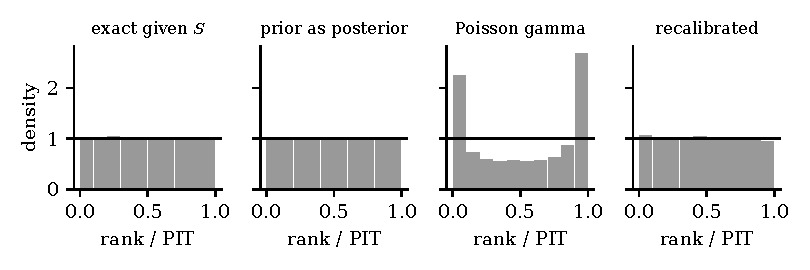
\includegraphics{figures/coal_sbc.pdf}
\caption{Histograms of the probability integral transform for the four posteriors of Example~\ref{coal:ex:sbc}. The first two are uniform, although only the first uses the data; the third is U shaped because the approximation is overconfident; the fourth is flat after recalibration, although its coverage still varies with $S$.}
\label{coal:fig:sbc}
\end{figure}

Example~\ref{coal:ex:sbc} is the networks' situation in miniature. Uniform ranks are necessary for a correct posterior but nowhere near sufficient, and a marginal repair can make the histogram look right while leaving the conditional error in place. The diagnostic that matters is calibration conditional on the data, which here is coverage within strata of $S$, and the corresponding repair must also depend on the data.

\section{Limitations}\label{coal:sec:limits}

This section collects what the chapter does not establish.

\begin{enumerate}
\item Theorem~\ref{coal:thm:geom} assumes constant population size, no recombination and no selection. The geometric decomposition uses the exponential holding times of \eqref{coal:eq:times} directly and does not survive a time change, though by Proposition~\ref{coal:prop:general} the mixed Poisson representation does, which is what Section~\ref{coal:sec:reference} exploits.

\item Proposition~\ref{coal:prop:notsuff} is made explicit by the three sequence calculation of Example~\ref{coal:ex:n3}, and Example~\ref{coal:ex:samesfs} computes exact likelihoods for two four sequence data sets. Beyond these small cases the full data likelihood is not computed, so the gap between spectrum based posteriors and the full data posterior is not measured; methods such as those of \citet{coal:griffiths1994} would be needed.

\item Proposition~\ref{coal:prop:hap} takes one step past the DeepSets ceiling, not the full step. The haplotype count is a scalar summary of linkage, and in Table~\ref{coal:tab:hap} it narrows the interval given $S$ by about 9\% at low diversity and 5\% at high diversity, but narrows the interval given the spectrum by at most 1.3\%, comparable to training variation. Encoders with genuine pairwise site features, or architectures on the inferred gene tree, remain unimplemented, and how far above the ceiling the full data posterior lies is unmeasured. This is the largest open gap in the chapter.

\item The reference posterior of Section~\ref{coal:sec:reference} validates the $S$ only encoder only. Because $\bm{\xi}$ is not a function of $L_n$, the same construction does not grade the spectrum encoders, which carry the chapter's main claims and remain validated by calibration alone.

\item The spectrum encoders undercover, at 0.877 to 0.891 against nominal 0.90 across Tables~\ref{coal:tab:const}, \ref{coal:tab:growth} and~\ref{coal:tab:hap}, so their width advantages over the $S$ based encoders are partly overconfidence. Only comparisons between rows with matching coverage are clean.

\item The exact machinery of Section~\ref{coal:sec:exact} is verified at $n=500$, but every learned encoder is trained at $n=30$. At the sample sizes of modern sequencing studies the spectrum has thousands of cells and the fixed width network used here would need replacing, most likely by an architecture exploiting the smoothness of $\E[\xi_i]=\theta/i$ in $i$.

\item Section~\ref{coal:sec:repair} applies the standard recalibration fix to the $S$ only network of Section~\ref{coal:sec:reference}: it repairs the marginal ranks but cannot reach the small conditional error that remains, which Example~\ref{coal:ex:sbc} reproduces exactly at a larger scale. We have not applied it to the spectrum maps, whose failures are far larger, and we do not implement conditional recalibration for the networks, so the calibration gap is characterised but still open.

\item Section~\ref{coal:sec:gbc} reports marginal posteriors only. The autoregressive construction \eqref{coal:eq:autoreg} for the joint law of $(\theta,g)$ is described but not evaluated, so nothing here speaks to the posterior dependence between mutation rate and growth rate, which is precisely the confounding the spectrum is supposed to resolve.
\end{enumerate}

\section{Discussion}\label{coal:sec:discussion}

Chapter~\ref{ch:suff} found that Kingman's exchangeable partitions hand generative computation an exactly sufficient statistic, reducing posterior inference to a two dimensional transport problem. The natural expectation was that his coalescent would do the same, with segregating sites in place of blocks. Corollary~\ref{coal:cor:duality} shows how close the two models are, placing them on one probability space with the partition as the thresholded coalescent, and Proposition~\ref{coal:prop:hapewens} shows that the observed haplotype partition is itself an Ewens partition. All of these statistics carry the same leading Fisher information $\theta^{-1}\log n$. Proposition~\ref{coal:prop:notsuff} shows the models nonetheless part company for inference, because the coalescent hides a genealogy that conditioning on $S$ does not integrate away, and Example~\ref{coal:ex:n3} shows this already with three sequences and one segregating site.

That failure is the reason the field built approximate Bayesian computation on this model and not on the Ewens formula. What generative computation changes is the response to it. Rather than choosing summaries and accepting parameter draws whose summaries fall close to the observed values, one learns a transport map by minimising check loss over prior predictive draws, and obtains the whole posterior quantile function. Theorem~\ref{coal:thm:deepsets} then supplies something that the summary selection literature could not: a proof of what a given class of learned summaries can see. Per site DeepSets encoders see the spectrum and nothing more, so the choice between hand chosen and learned summaries is, within that class, not a choice at all.

The ceiling is real but, in the designs tested here, low. Proposition~\ref{coal:prop:hap} names a single scalar outside the class, and Example~\ref{coal:ex:samesfs} shows it moving the posterior for data sets the spectrum cannot tell apart. In Table~\ref{coal:tab:hap} the haplotype count adds substantially to $S$, but at most 1.3 percent to the full spectrum. The two observations are compatible: Example~\ref{coal:ex:samesfs} conditions on one spectrum and varies the haplotypes, whereas the experiment averages over the prior predictive, where most of what $H$ says about the tree is already said by the shape of the spectrum. The useful reading is that a scalar is not enough, and that further gains must come from features that see which sequences share which mutations, as in the pairwise statistic noted after Example~\ref{coal:ex:samesfs}, which is where the genuinely linked information lives.

The obvious next step is therefore to go past a scalar. Corollary~\ref{coal:cor:coarse} identifies the gene tree as the maximal invariant, which suggests encoding the inferred perfect phylogeny directly and learning on trees rather than on counts. Whether the resulting posteriors close the gap to the full data likelihood, and whether they survive simulation based calibration at the replicate counts used here, are questions our experiments raise and do not answer. Proposition~\ref{coal:prop:general} already supplies the grading instrument for one half of that programme: since the likelihood of $S$ under any demography is a one dimensional integral against the tree length law, exact reference posteriors are available for arbitrary population histories, and Section~\ref{coal:sec:reference} uses one. Extending the same idea past $S$ is the obstacle, because the spectrum is not a functional of tree length alone.

A last word on calibration. Section~\ref{coal:sec:repair} reports a repair that passes the marginal test, and we think what it leaves untouched is the more useful finding. Rank recalibration is the reflexive response to a nonuniform simulation based calibration histogram, and it is guaranteed to flatten the histogram, up to the noise of the calibration set, whatever the map does for particular data. For the $S$ only network it did so, removing a common overcoverage, and left the spread of coverage across strata of $S$ where it was, because that error varies with the data rather than across the board. Example~\ref{coal:ex:sbc} shows the same thing with every posterior known exactly and a much larger conditional error, and also shows the converse hazard, that a posterior which ignores the data passes the test. Practitioners reaching for the standard fix should check calibration conditional on the data as well, because a flat histogram after recalibration is guaranteed and therefore says nothing about the conditional regime.

\subsection*{Reproducibility}

The exact mass function of Theorem~\ref{coal:thm:geom} is obtained by a 4096 point fast Fourier transform of the generating function, or by the convolution recursion after Corollary~\ref{coal:cor:exact}. The coalescent simulator accumulates branch length by leaf count class using a flattened bin count, and is validated against $\E[\xi_i]=\theta/i$ and, at $n=4$, against the exact law of Table~\ref{coal:tab:n4}. Quantile networks are implemented in numpy with hand coded backpropagation of the check loss. Code for the worked examples and for Tables~\ref{coal:tab:exact} to~\ref{coal:tab:reference} is in the directory \texttt{code/coal\_rev} accompanying the book.

\section{Exercises}\label{coal:sec:exercises}

\begin{enumerate}[label=\arabic*., leftmargin=*]
\item Show that $\Prob(S=0)=(n-1)!/\{(\theta+1)\cdots(\theta+n-1)\}$, that this equals the Ewens probability $\Prob(K_n=1)$, and that it equals $1/n$ when $\theta=1$.
\emph{Hint.} $S=0$ if and only if every $S_k=0$; for the Ewens side use the Feller coupling.

\item For $n=4$ and $\theta=1$ verify $\Prob(S=2)=115/576$ in two ways: from the complete homogeneous polynomial $h_2(\tfrac12,\tfrac13,\tfrac14)$, and from \eqref{coal:eq:tavare}.
\emph{Hint.} $h_2=\sum_kq_k^2+\sum_{j<k}q_jq_k=115/144$.

\item Show that $\E[S(S-1)]=\theta^2\{a_1(n)^2+a_2(n)\}$ and deduce that \eqref{coal:eq:varhat} is unbiased for $\Var(\hat\theta_W)$.
\emph{Hint.} Use \eqref{coal:eq:watterson} and $\E[S(S-1)]=\Var(S)+\E[S]^2-\E[S]$.

\item Prove that $S$ is stochastically increasing in $\theta$, and hence that the exact interval of Section~\ref{coal:sec:wattex} has at least the stated coverage.
\emph{Hint.} Each $S_k$ is geometric with failure probability $\theta/(\theta+k-1)$, increasing in $\theta$; couple the summands monotonically.

\item For $n=3$ derive the full law of the spectrum, $\Prob(\xi_1=i,\xi_2=j)=\E\bigl[\coalPois(i;\theta(3T_3+T_2)/2)\,\coalPois(j;\theta T_2/2)\bigr]$, and recover the formula of Example~\ref{coal:ex:n3} for $\Prob(\xi_2=1\mid S=1)$.
\emph{Hint.} Here $\ell_1=3T_3+T_2$ and $\ell_2=T_2$; condition on the tree and use the tilted exponential moments.

\item In Example~\ref{coal:ex:samesfs}, show that the conditional probability of data set A given $\bm\xi=(2,0,0)$ tends to $1/2$ as $\theta\to0$.
\emph{Hint.} At $\theta=0$ the tilt disappears; compute $\E[\sum_je_j^2]$ and $\E[\sum_{i<j}e_ie_j]$ for both topologies from $\E[T_k]=2/\{k(k-1)\}$ and $\E[T_k^2]=8/\{k(k-1)\}^2$.

\item Show that $H$ and $K'=1+\#\{k:S_k\ge1\}$ always agree when $n=2$, and construct a genealogy with mutations for $n=3$ on which $K'=3$ but $H=2$.
\emph{Hint.} For $n=3$ put one mutation on the lone lineage in each of the two epochs.

\item Prove the identity $I_{\bm S}(\theta)=\theta^{-1}\sum_{k=2}^n(\theta+k-1)^{-1}$ by computing the score of the geometric directly in $\theta$, and check the entry $1.083$ of Table~\ref{coal:tab:info} for $n=4$, $\theta=1$.
\emph{Hint.} $\tfrac12+\tfrac13+\tfrac14=\tfrac{13}{12}$.

\item Show that a pairwise encoder $\sum_{j<l}\psi(x_j,x_l)$ with $\psi$ invariant under simultaneous permutation of the lineages in both arguments can distinguish the two data sets of Example~\ref{coal:ex:samesfs}, and so is not bound by Theorem~\ref{coal:thm:deepsets}.
\emph{Hint.} Take $\psi(x,y)=\coalind\{x=y\}$.

\item Prove that if a candidate posterior for $\theta$ ignores the data and equals the prior, its probability integral transform is exactly uniform under the prior predictive, so simulation based calibration cannot reject it.
\emph{Hint.} $F_\pi(\theta)$ is uniform when $\theta\sim\pi$ and $F_\pi$ is continuous.

\item Derive the rescaled time $\Lambda(t)=(e^{gt}-1)/g$ for $N(t)=N_0e^{-gt}$ and show that the expected time to the most recent common ancestor of two sequences is $g^{-1}\E[\log(1+gE)]$ with $E\sim\coalExp(1)$; evaluate it numerically for $g=1$.
\emph{Hint.} The value is $e\,E_1(1)\approx0.596$, where $E_1$ is the exponential integral.

\item Using the convolution recursion after Corollary~\ref{coal:cor:exact}, compute the exact posterior of $\theta$ given $S=18$ and $n=11$ under the prior $\pi(\theta)\propto1/\theta$ and compare its 90\% interval with the exact confidence interval of Example~\ref{coal:ex:watterson}.
\emph{Hint.} The answers should be close to $(2.97,14.31)$ and $(2.97,15.05)$.
\end{enumerate}

\begin{thebibliography}{99}

\bibitem[Beaumont et~al.(2002)]{coal:beaumont2002}
Beaumont, M. A., Zhang, W. and Balding, D. J. (2002). Approximate Bayesian computation in population genetics. \emph{Genetics} 162, 2025 to 2035.

\bibitem[Ewens(1972)]{coal:ewens1972}
Ewens, W. J. (1972). The sampling theory of selectively neutral alleles. \emph{Theoretical Population Biology} 3, 87 to 112.

\bibitem[Felsenstein(1992)]{coal:felsenstein1992}
Felsenstein, J. (1992). Estimating effective population size from samples of sequences: inefficiency of pairwise and segregating sites as compared to phylogenetic estimates. \emph{Genetical Research} 59, 139 to 147.

\bibitem[Fu(1995)]{coal:fu1995}
Fu, Y. X. (1995). Statistical properties of segregating sites. \emph{Theoretical Population Biology} 48, 172 to 197.

\bibitem[Griffiths and Tavar\'e(1994)]{coal:griffiths1994}
Griffiths, R. C. and Tavar\'e, S. (1994). Simulating probability distributions in the coalescent. \emph{Theoretical Population Biology} 46, 131 to 159.

\bibitem[Kingman(1977)]{coal:kingman1977}
Kingman, J. F. C. (1977). The population structure associated with the Ewens sampling formula. \emph{Theoretical Population Biology} 11, 274 to 283.

\bibitem[Kingman(1982)]{coal:kingman1982}
Kingman, J. F. C. (1982). The coalescent. \emph{Stochastic Processes and their Applications} 13, 235 to 248.

\bibitem[Kreitman(1983)]{coal:kreitman1983}
Kreitman, M. (1983). Nucleotide polymorphism at the alcohol dehydrogenase locus of \emph{Drosophila melanogaster}. \emph{Nature} 304, 412 to 417.

\bibitem[Polson, Ruggeri and Sokolov(2024)]{coal:polson2024}
Polson, N. G., Ruggeri, F. and Sokolov, V. (2024). Generative Bayesian computation for maximum expected utility. \emph{Entropy} 26, 1076.

\bibitem[Tajima(1989)]{coal:tajima1989}
Tajima, F. (1989). Statistical method for testing the neutral mutation hypothesis by DNA polymorphism. \emph{Genetics} 123, 585 to 595.

\bibitem[Talts et~al.(2018)]{coal:talts2018}
Talts, S., Betancourt, M., Simpson, D., Vehtari, A. and Gelman, A. (2018). Validating Bayesian inference algorithms with simulation based calibration. arXiv:1804.06788.

\bibitem[Tavar\'e(1984)]{coal:tavare1984}
Tavar\'e, S. (1984). Line of descent and genealogical processes, and their applications in population genetics models. \emph{Theoretical Population Biology} 26, 119 to 164.

\bibitem[Tavar\'e et~al.(1997)]{coal:tavare1997}
Tavar\'e, S., Balding, D. J., Griffiths, R. C. and Donnelly, P. (1997). Inferring coalescence times from DNA sequence data. \emph{Genetics} 145, 505 to 518.

\bibitem[Watterson(1975)]{coal:watterson1975}
Watterson, G. A. (1975). On the number of segregating sites in genetical models without recombination. \emph{Theoretical Population Biology} 7, 256 to 276.

\bibitem[Zaheer et~al.(2017)]{coal:zaheer2017}
Zaheer, M., Kottur, S., Ravanbakhsh, S., P\'oczos, B., Salakhutdinov, R. and Smola, A. (2017). Deep sets. In \emph{Advances in Neural Information Processing Systems} 30.

\end{thebibliography}
